\documentclass[12pt]{article}

\usepackage{amsmath,amssymb,amsthm}
\usepackage[T1]{fontenc}
\usepackage{graphics}
\usepackage{qtree}
\usepackage{tikz}
\usepackage[utf8]{inputenc} % æøå
\usepackage[T1]{fontenc} % mere æøå
\usepackage[danish]{babel} % orddeling
\usepackage{verbatim} % så man kan skrive ren tekst
\usepackage[all]{xy} % den sidste (avancerede) formel i dokumentet
\usepackage{fullpage} % mindre margin

\title{ProjDat 2014\\Props 2.0}
\author{Louise Knudsen (140791 - zsh845)\\
Helena Bach (180492 - wzg314)\\
David Pedersen (060890 - tlb209)\\\\
Instructor: Simon Shine }
\date{\today}

\newcommand{\R}{\mathbb{R}}
\newcommand{\C}{\mathbb{C}}
\newcommand{\N}{\mathbb{N}}
\newcommand{\Z}{\mathbb{Z}}
\newcommand{\Q}{\mathbb{Q}}

\newcommand{\og}{\wedge}

\begin{document}
\maketitle
\newpage
\section*{Literature review}
\subsection*{Designing for Usability: Key Principles and What Designers Think}
The article is written in 1985, and gives a theoretical and empirical view on software engineering, and the conflict in how designers think of a good development-process and what they actual do while developing a system. The article focusses on three principles of system design: \\\\
1) Early and continual focus on users. The key point here, is to reach a understanding of who the users will be, at a very early state in the project. \\\\
2) Empirical measurement of usage. At this stage, still at a early state, observe, record and analyse users performances and reactions in using simulations and prototypes of the system.\\\\
3) Iterative design. Modify, test and modify the system repeatedly throughout the development-process according to the observations of the measurement of usage. \\\\
The empirical part of the article focuses on what designers, programmers and developers think the five (or so) major steps in system-developing should be, prior being introduced to the three principles the article recommend. Furthermore it focuses on the conflict between how many designers believe these three principles to be obvious, and the fact that less than 20 \% of the designers asked mentioned all three principles as the major steps to go through while developing a new computer system for end users. \\\\
The three principles mentioned in the article well agrees with our project development-process so far, as we have focused a lot on meeting several times with the client, to ensure we meet and discuss, both the current and the new system, with all the different actors who will be using the system, prior to the coding begins. We also intend to use the client in testing of prototypes and simultaneously modify our system and thereby quickly fix potential flaws observed during the testing.
\subsection*{A Rational Design Process: How and Why to Fake It}

This article is written in 1986. It starts giving arguments for why some sort of rational process is required when designing software even though it is hard. It then goes into describing what the authors thinks such a process looks like.
First of all, they describe the importance of a requirements document, and argue that the most efficient way of organizing the document is:\\
a) Computer specification\\
b) Input/output interfaces\\
c) Specification of output values\\
d) Timing constraints\\
e) Accuracy constraints\\
f) Likely changes\\
g) Undesired event handling\\\\ 
They argue that you should divide the project into small work assignments, which they refer to as modules. Documentation,including specifications of the interfaces and internal structures, should be written for each module. This is then put together into a tree-structured module guide.\\
This will avoid duplication and gaps. It will achieve separation of concerns and most important, help ignorant maintainers to find out which modues are affected by a problem report or change request, and therefore be useful as long as the software is used.\\\\
The author outlines reasons that the documentation today (30 years ago), doesn't get used. This is because of poor organisation, boring prose, confusing and inconsistent terminology and most documentation is written in the end of the project, which leads to documentation only useful to people who know the system well.\\
By creating the documentation iteratively you can ensure that it is always up to date, follows the structure of the implementation and is consistent.\\\\
The authors points out that building a system on these terms is very difficult and time consuming in the short run. However the rational process, even faking it by rewriting the documentation during the process, will result in a product that can be understood, maintained and reused.\\\\
\textit{'If the project is worth doing, the methods described here are worth using'}

\section*{IT-project development}
\section{Abstract}
\textit{The Royal Danish Theatre's props department uses a locally installed database-system to search through all of the props and productions and their corresponding set-up- and run-lists. The system was developed more than 20 years ago by their own Claus Nepper Fakkenberg. Claus alone holds the responsibility for maintaining the system, as he is the only one who understands the source-code, which will soon be a problem as he is now retiring. \\
Due to the age of the system, some functionalities are no longer needed, and there are new requirements that are not implemented, most importantly a need to use the system outside of the office. Our project will therefore be to develop a web-based database-system for the props department, to replace the current system.}
\section{Project purpose and scope}
A web-based database-system of The Royal Danish Theatre props department. The system should primarily be a searching tool used to prepare and run performances and search for props in current and previous productions by the assistant stage managers, and secondly be used for budget monitoring, search for supplier information as well as keeping track of all performance information, by the chairman of the props department. The system should be usable for people with greatly variable computer experience.
\subsection{Definitions}
The Royal Danish Theatre uses a lot of different terms in their work, and some of these should also be used in the future database system. The terms we have been presented to so far are listed with a short description below: \\
Every production has a unique 8-digit number, containing of 4 random digits followed by a dash and premiere-year for this particular production. (There can be multiple productions of, for instance the same play, which then have different premiere-years) \\
If a production is \textit{SKILT}, it means that it has been discarded and the props are back in the storage room. \\
If a production is \textit{I REPERTOIRE}, it is being played in the current season and the props are in use. \\
If the production is \textit{I CONTAINER} or similar, the production is not yet \textit{SKILT} nor is it currently being played, and the props are therefore occupied but not in use.
\subsection{The FACTOR Criterion}
\begin{description}
  \item[Functionality:] Keeping track of the props and performances, and help in running these. As well as support the administration.
  \item[Application domain:] The Royal Danish Theatre.
  \item[Conditions:] The system should be usable by multiple user at a time, wherever there are access to the internet.
  \item[Technology:] The system will be developed on standard laptops, and should be usable on standard PC's and tablets and supported by every OS.
  \item[Object:] Props, pictures and employees in the props department.
  \item[Responsibility:] Searching and administrative tool.
\end{description}
\section{Requirement Elicitation}
\subsection{a)}
\subsubsection{Nonfunctional Requirements}
\begin{itemize}
  \item The system should be web-based and usable on standard PC's and tablets, and supported by every OS.
  \item The webapplication should be user friendly and easy to navigate. The most commonly used functionalities, namely the so-called run- and set-up-lists should be preferable be found on the frontpage.
  \item It should be possible for Martin (head of the IT-department) to maintain and support, and possibly expand the system after product-delivery. Therefore the system will be developed using MySQL and PHP, which is familiar to Martin.
  \item The system should be able to communicate with the existing media-database Cumulus.
  \item The system should be secure in a way that prevents people from the outside to corrupt the data.
  \item The interface should be in Danish.
  \item It should be made in such a way that makes it easy to extend with additonal functionality.
\end{itemize}
\subsubsection{Functional Requirements}
\begin{itemize}
  \item It should be possible to do cross search for props, productions, and suppliers.
  \item It should be possible to add, edit and delete props, productions, and suppliers.
  \item It should be possible to print run- and set-up-lists.
\end{itemize}
\subsection{b) UML use case diagram}
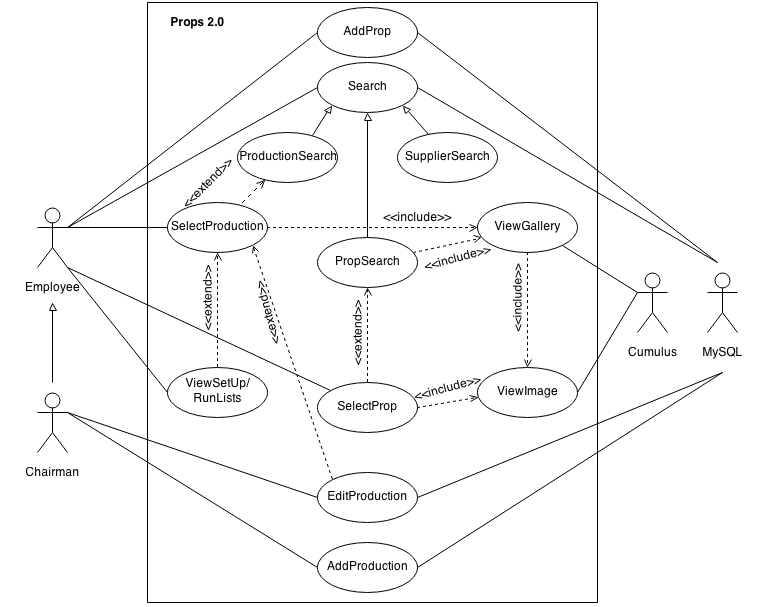
\includegraphics[scale=0.6]{use.png}\\
We have four actors in our use case diagram:
\begin{itemize}
\item An employee, who has permission to add a prop, search for props/productions/suppliers, and view this items, indicated with the lines from \textit{Employee} to the different use cases. The arrows between the use cases indicate an interaction between them - the employee can "activate" such an use case during another use case or going directly to the use case.
\item A Chairman, who is an extension of an employee, with the special permissions to edit and add productions.
\item A MySQL database, which holds the props/productions/suppliers data the \textit{Employee} and \textit{Chairman} actors accesses in the different use cases.
\item A Cumulus media database, which holds the image data the \textit{Employee} and \textit{Chairman} actors accesses in these use cases. 
\end{itemize}
\subsection{c) Use cases}
The following three use cases are the ones of most importance:
%1. Tilføj Rek
\[
\begin{array}{ll}
\hline
\textit{Use case name} & \texttt{AddProp} \\
\hline
\textit{Participating actors} & \text{Initiated by \texttt{Employee}} \\
& \text{Communicates with \texttt{MySQL}} \\
\hline
\textit{Flow of events} & 
\begin{array}{l}
\text{1. The \texttt{Employee} activates the "Add prop"  function.}\\
\quad \quad \quad \text{2. \texttt{Props 2.0} responds by presenting a form to the \texttt{Employee}.} \\
\text{3. The \texttt{Employee} fills out the form with the relevant prop-info,} \\ \quad \text{and submits it.} \\
\quad \quad \quad \text{4. \texttt{Props 2.0} receives the form, and the MySQL database} \\ \quad \quad \quad \quad \text{gets updated. \texttt{Props 2.0} displays a confirmation of the}\\ \quad \quad \quad \quad \text{update.}
\end{array} \\
\hline
\textit{Entry condition} & \text{The \texttt{Employee} must be logged into the Theatre's Wi-Fi} \\
\hline
\textit{Exit condition} & \text{The \texttt{Employee} has received a confirmation OR} \\ & \text{An explanation indicating why the transaction could not be processed.} \\
\hline
\textit{Quality requirements} & \text{Not yet defined} \\
\hline
\end{array}
\]
%2. Tilføj forestilling
\\\\
\[
\begin{array}{ll}
\hline
\textit{Use case name} & \texttt{AddProduction} \\
\hline
\textit{Participating actors} & \text{Initiated by \texttt{Chairman}} \\
& \text{Communicates with \texttt{MySQL}} \\
\hline
\textit{Flow of events} & 
\begin{array}{l}
\text{1. The \texttt{Chairman} activates the "Add production" function.}\\
\quad \quad \quad \text{2. \texttt{Props 2.0} responds by presenting a form to the \texttt{Chairman}.} \\
\text{3. The \texttt{Chairman} fills out the form with the relevant production-info,} \\ \quad \text{and submits it.} \\
\quad \quad \quad \text{4. \texttt{Props 2.0} receives the form, and the MySQL database} \\ \quad \quad \quad \quad \text{gets updated. \texttt{Props 2.0} displays a confirmation of the}\\ \quad \quad \quad \quad \text{update.}
\end{array} \\
\hline
\textit{Entry condition} & \text{The \texttt{Chairman} must be logged into the Theatre's Wi-Fi} \\
\hline
\textit{Exit condition} & \text{The \texttt{Chairman} has received a confirmation OR} \\ & \text{An explanation indicating why the transaction could not be processed.} \\
\hline
\textit{Quality requirements} & \text{Not yet defined}\\
\hline
\end{array}
\]
%3. Søg
\\\\
\[
\begin{array}{ll}
\hline
\textit{Use case name} & \texttt{Search} \\
\hline
\textit{Participating actors} & \text{Initiated by \texttt{Employee}} \\
& \text{Communicates with \texttt{MySQL}} \\
\hline
\textit{Flow of events} & 
\begin{array}{l}
\text{1. The \texttt{Employee} activates the "Search" function.}\\
\quad \quad \quad \text{2. \texttt{Props 2.0} responds by presenting a form to the \texttt{Employee}.} \\
\text{3. The \texttt{Employee} fills out the form with the search criteria,} \\ \quad \text{and submits it.} \\
\quad \quad \quad \text{4. \texttt{Props 2.0} receives the form, the MySQL database} \\ \quad \quad \quad \quad \text{returns the matching data and \texttt{Props 2.0} displays it}
\end{array} \\
\hline
\textit{Entry condition} & \text{The \texttt{Employee} must be logged into the Theatre's Wi-Fi} \\
\hline
\textit{Exit condition} & \text{The \texttt{Employee} has received a list of matching data OR} \\ & \text{A "No match"  message} \\
\hline
\textit{Quality requirements} & \text{Not yet defined} \\
\hline
\end{array}
\]
%4. Vælg rek
\\
We have in addition made use cases, explaining the rest of the actions in the UML use case diagram: \\
\[
\begin{array}{ll}
\hline
\textit{Use case name} & \texttt{SelectProp} \\
\hline
\textit{Participating actors} & \text{Initiated by \texttt{Employee}} \\
\hline
\textit{Flow of events} & 
\begin{array}{l}
\text{1. The \texttt{Employee} selects a prop from the results of a premade search} \\
\quad \quad \quad \text{2. \texttt{Props 2.0} responds by presenting a more detailed}\\ \quad \quad \quad \quad \text{description of the prop to the \texttt{Employee}.}
\end{array} \\
\hline
\textit{Entry condition} & \text{This use case extends the  \texttt{PropSearch} use case} \\
\hline
\textit{Exit condition} & \text{The \texttt{Employee} is looking at the prop description} \\
\hline
\textit{Quality requirements} & \text{This use case includes the \texttt{ViewImage} use case} \\
\hline
\end{array}
\]
%5. Vælg forestilling:\\
\\\\
\[
\begin{array}{ll}
\hline
\textit{Use case name} & \texttt{SelectProduction} \\
\hline
\textit{Participating actors} & \text{Initiated by \texttt{Employee}} \\
\hline
\textit{Flow of events} & 
\begin{array}{l}
\text{1. The \texttt{Employee} selects a production from the results of a premade}\\ \quad \text{search}\\
\quad \quad \quad \text{2. \texttt{Props 2.0} responds by presenting a more detailed}\\
\quad \quad \quad \quad \text{description of the production to the \texttt{Employee}.}
\end{array} \\
\hline
\textit{Entry condition} &
\text{This use case extends the \texttt{ProductionSearch} use case.}\\
\hline
\textit{Exit condition} & \text{The \texttt{Employee} is looking at the production information.} \\
\hline
\textit{Quality requirements} & \text{This use case includes the \texttt{ViewGallery} use case.} \\
\hline
\end{array}
\]
%6. Køre/opstil
\\\\
\[
\begin{array}{ll}
\hline
\textit{Use case name} & \texttt{ViewSetUp/RunLists} \\
\hline
\textit{Participating actors} & \text{Initiated by \texttt{Employee}} \\
\hline
\textit{Flow of events} & 
\begin{array}{l}
\text{1. The \texttt{Employee} selects the list from the results of a production} \\ \quad \text{search} \\
\quad \quad \quad \text{2. \texttt{Props 2.0} responds by presenting the list to the}\\ \quad \quad \quad \quad \texttt{Employee.}
\end{array} \\
\hline
\textit{Entry condition} & \text{This use case extends the  \texttt{SelectProduction} use case} \\
\hline
\textit{Exit condition} & \text{The \texttt{Employee} is looking at the list} \\
\hline
\textit{Quality requirements} & \text{Not yet defined} \\
\hline
\end{array}
\]
%7. Redigér/slet
\\\\
\[
\begin{array}{ll}
\hline
\textit{Use case name} & \texttt{EditProduction} \\
\hline
\textit{Participating actors} & \text{Initiated by \texttt{Chairman}} \\
& \text{Communitates with \texttt{MySQL}} \\
\hline
\textit{Flow of events} & 
\begin{array}{l}
\text{1. The \texttt{Chairman} activates the "Edit production" function} \\
\quad \quad \quad \text{2. \texttt{Props 2.0} responds by presenting a form to the \texttt{Chairman}}\\
\text{3. The \texttt{Chairman} fills out the form and submit the changes OR} \\ \quad \text{The \texttt{Chairman} selects the "Delete" option} \\
\quad \quad \quad \text{4. \texttt{Props 2.0} receives the form, and the MySQL database} \\ \quad \quad \quad \quad \text{gets updated. \texttt{Props 2.0} displays a update- OR}\\\quad \quad \quad \quad \text{delete-comfirmation} 
\end{array} \\
\hline
\textit{Entry condition} & \text{This use case extends the  \texttt{SelectProduction} use case} \\
\hline
\textit{Exit condition} & \text{The \texttt{Chairman} has received a confirmation OR} \\ & \text{An explanation indicating why the transaction could not be processed.} \\
\hline
\textit{Quality requirements} & \text{Not yet defined} \\
\hline
\end{array}
\]
%8. Se Galleri:
\\\\
\[
\begin{array}{ll}
\hline
\textit{Use case name} & \texttt{ViewGallery} \\
\hline
\textit{Participating actors} & \text{Initiated by \texttt{Employee}}\\ &
\text{Communicates with \texttt{Cumulus}}\\
\hline
\textit{Flow of events} & 
\begin{array}{l}
\text{1. The \texttt{SelectProduction} or \texttt{PropSearch} use case gets evoked}\\
\quad \quad \quad \text{2. \texttt{Props 2.0} requests \texttt{Cumulus} for the image data}\\
3.\text{\texttt{Cumulus} returns the matching images}\\
\quad \quad \quad \text{4. \texttt{Props 2.0} responds by presenting the images as a gallery}
\end{array} \\
\hline
\textit{Entry condition} &
\text{The \texttt{Employee} must initiate the \texttt{SelectProduction} or \texttt{PropSearch}}\\ &
\text{use case to initiate this use case}\\
\hline
\textit{Exit condition} & \text{The \texttt{Employee} is looking at the gallery.} \\
\hline
\textit{Quality requirements} & \text{This use case includes the \texttt{ViewImage} use case.} \\
\hline
\end{array}
\]
%9. Se billede:
\\\\
\[
\begin{array}{ll}
\hline
\textit{Use case name} & \texttt{ViewImage} \\
\hline
\textit{Participating actors} & \text{Initiated by \texttt{Employee}}\\ &
\text{Communicates with \texttt{Cumulus}}\\
\hline
\textit{Flow of events} & 
\begin{array}{l}
\text{1. The \texttt{ViewGallery} or \texttt{SelectProp} use case gets evoked}\\
\quad \quad \quad \text{2. \texttt{Props 2.0} requests \texttt{Cumulus} for the image}\\
\text{3. \texttt{Cumulus} returns the matching image}\\
\quad \quad \quad \text{4. \texttt{Props 2.0} responds by presenting the image to the}\\ \quad \quad \quad \quad\texttt{Employee}
\end{array} \\
\hline
\textit{Entry condition} &
\text{The \texttt{Employee} must initiate the \texttt{ViewGallery} or \texttt{SelectProp} use}\\ &
\text{case to initiate this use case}\\
\hline
\textit{Exit condition} & \text{The \texttt{Employee} is looking at the image.} \\
\hline
\textit{Quality requirements} & \text{Not yet defined} \\
\hline
\end{array}
\]
\subsection{d) Class diagram}
Here is a class diagram of the model layer as we imagine it might look.
\newline
\newline
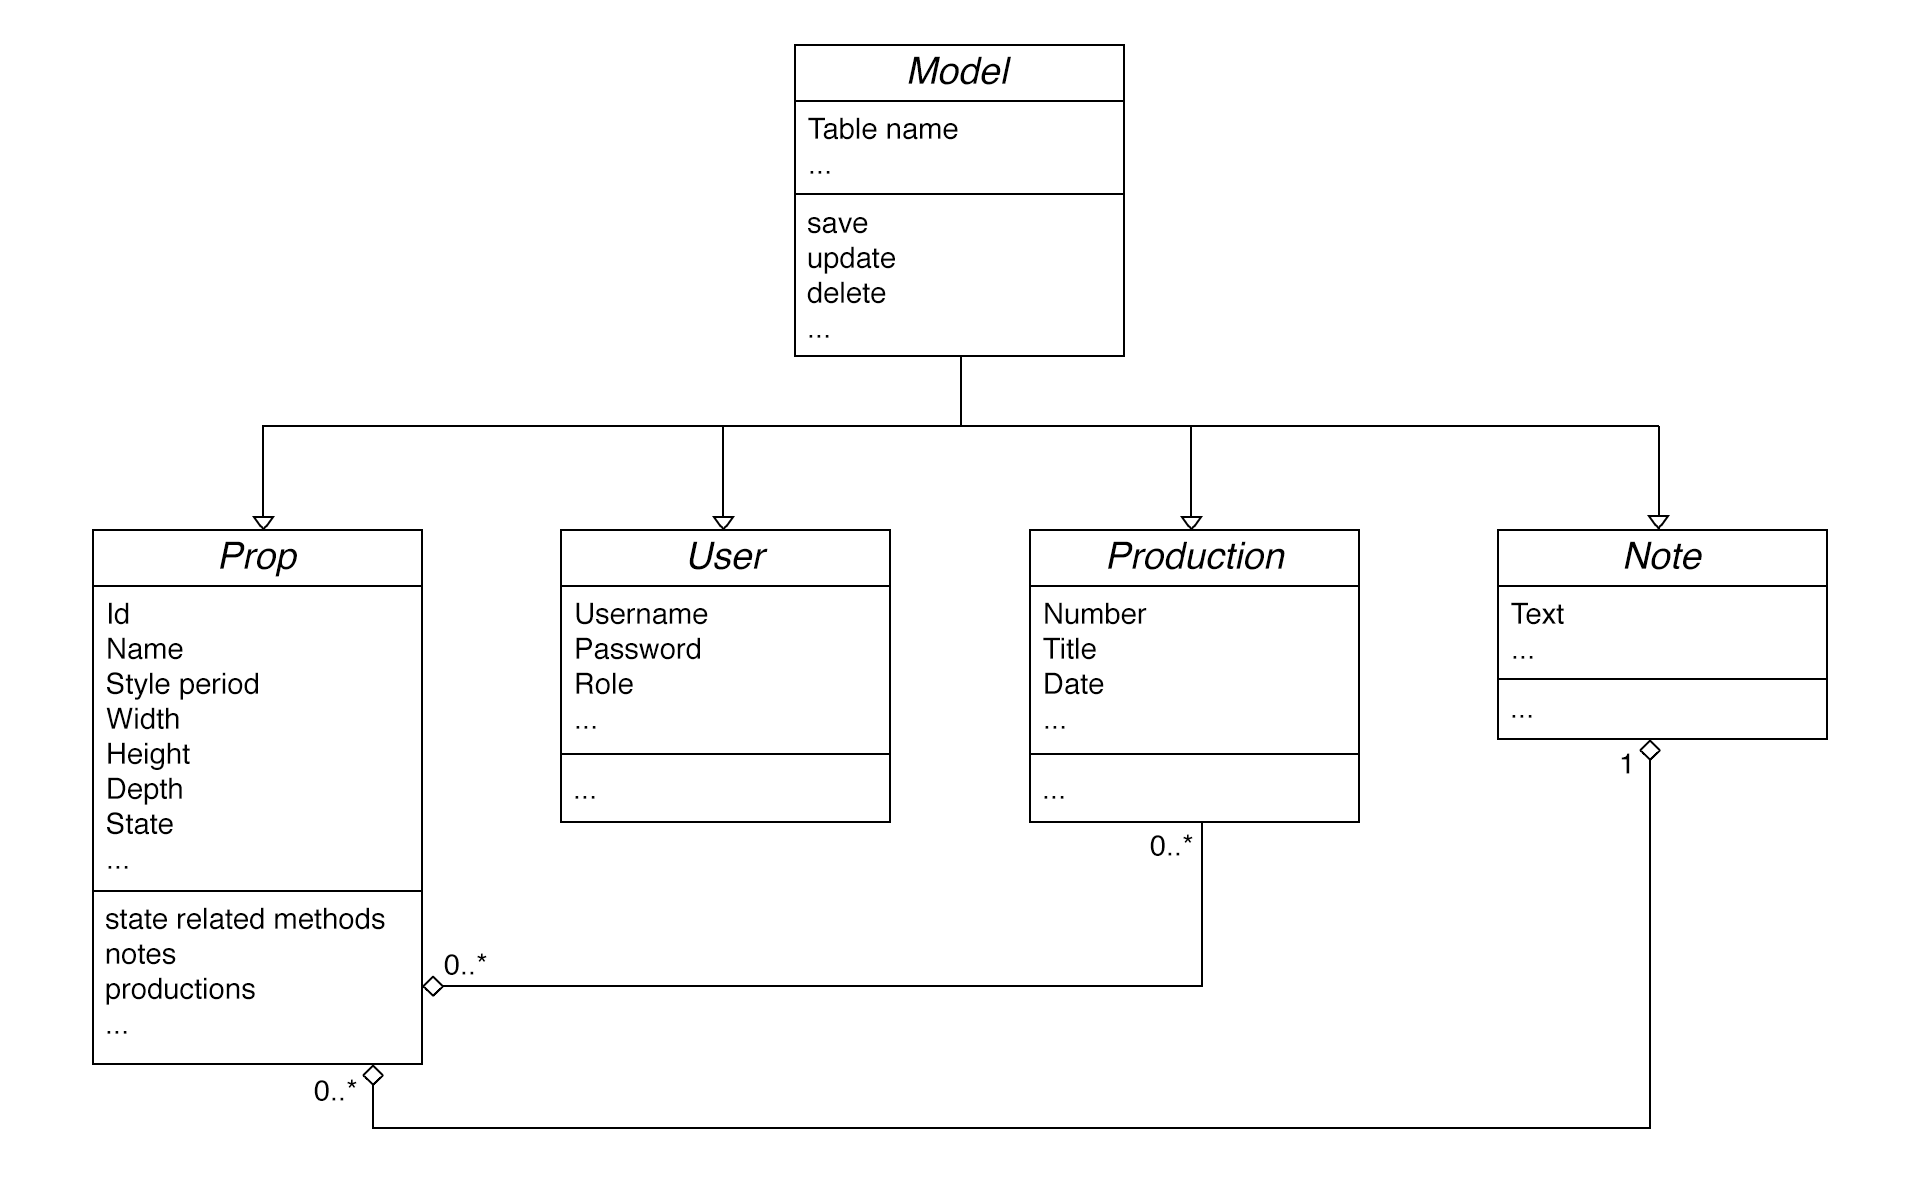
\includegraphics[scale=0.2]{class-diagram.png}
\newline
There will be one abstract model class that implements methods used by all models. There will then be subclasses of this model that implement the domain functionality.\\
They will be associated with each other in different ways. A prop will be associated with many productions and can have many notes. A production can have many props and a note belongs to exactly one prop.\\
There will then also be various attributes on the models that correspond to the database columns. The models will also have methods but at this point its hard to say specifically which methods they will need. The prop model will however most likely need methods for changing its state and accessing the other associated objects.
\subsection*{e) Sequence diagram}
We've chosen the use case of \texttt{AddProb}, \texttt{AddProject} and \texttt{Search} thus we think these are the main use cases of our webapplication.\\\\
Since we haven't made the object model yet, obviously we can't determine which objects we'll call in our sequence diagram. Therefore we've initially created the sequence diagram using the webpages that we do know we'll have. Iterative while investigating which objects are needed, we will then update and improve the sequence diagrams.\\\\
\textit{We're not sure how to represent the situation where the user's sending a request to the addProbPage about going back to the frontPage. And again same problem when the user's choosing a prob on the searchPage, which will then send the user to the propPage}\\\\
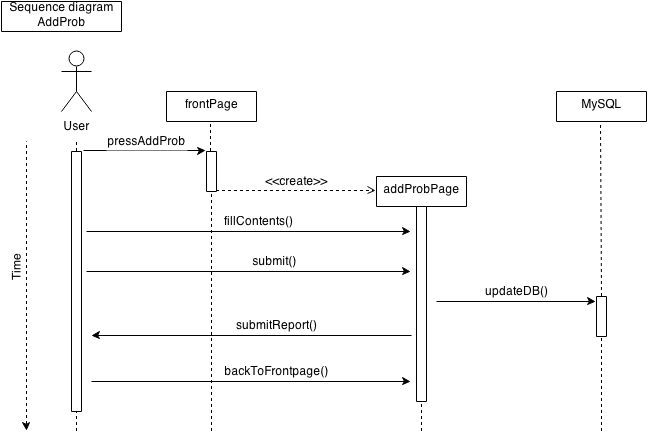
\includegraphics[scale=0.6]{sequenceDiagram_addProb.png}\\\\
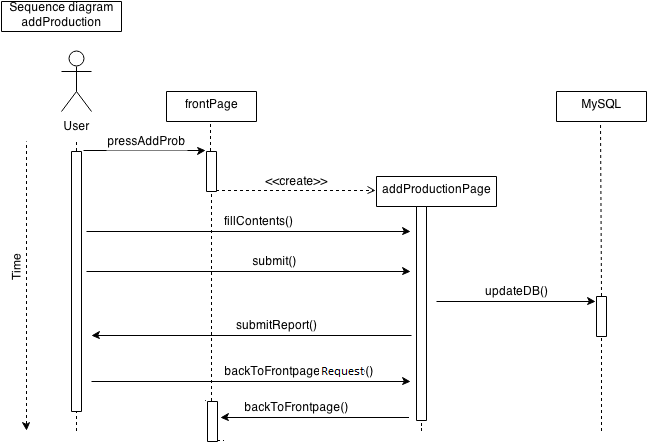
\includegraphics[scale=0.6]{sequenceDiagram_addProduction.png}\\\\
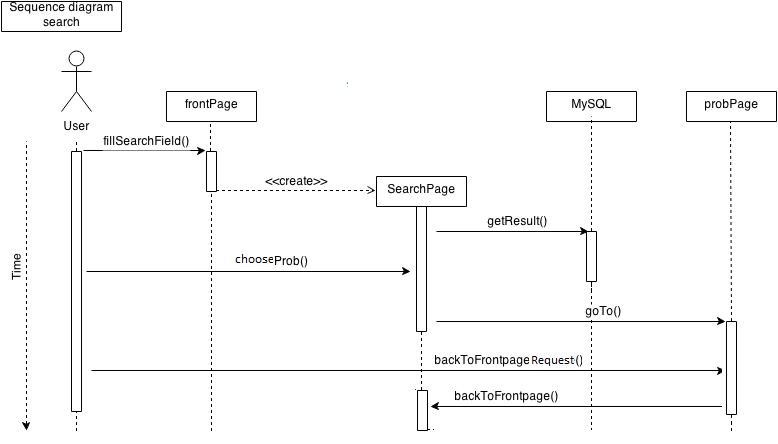
\includegraphics[scale=0.6]{sequenceDiagram_search.png}\\
\section{System-design summary}
Since we are developing a web application the software stack is mostly given. We will be developing the frontend using HTML, CSS, and JavaScript. This is the technologies that you have to use when deploying to the web.
\newline
For the backend you have a bit more freedom for choosing software stack. We have chosen to use PHP and MySQL as this will allow the theatre's IT department to continue maintaining the application after our final delivery.
\section{Program- and systemtest}
We've chosen to use Test Driven Development when developing the system. This means that tests will be written before the implementation code is written. This weaves the test plan and implementation plan together. There will not be a dedicated time period in which we do the testing and there will not be a defined set of resources (developers) in charge of doing the testing. This is because the testing will be done by the developers while they're writing the implementation code.
\newline
Our test suite will consist of both low level unit tests and high level feature tests. The unit tests will be focused on testing one unit of the system. A unit will mostly be a single class and the methods within it, and will focus on testing the side effects or return values of the methods. Unit tests will sometimes (not exclusively) be isolated from other units they interact with (boundaries). This will be done through mocks and stubs.
\newline
\newline
To ensure that all the units are interacting correctly and that the features of the application are actually working we will make use of high level feature tests. These tests will focus on driving the application from a user's point of view (the browser). They will do things like click links, fill out forms, and make assertions about what should appear on the screen. This will allow us to test something as high level as "A user creates a new prop and sees it on the front page".
\section{User interface and interaction design}
\subsection{a) Screenshots of user interfaces}
% (a) Præsenter skærmbilleder af de mest interessante dele af jeres brugergrænseflade.
The following are screenshots of our most recent prototype.
\newline
\newline
\centerline{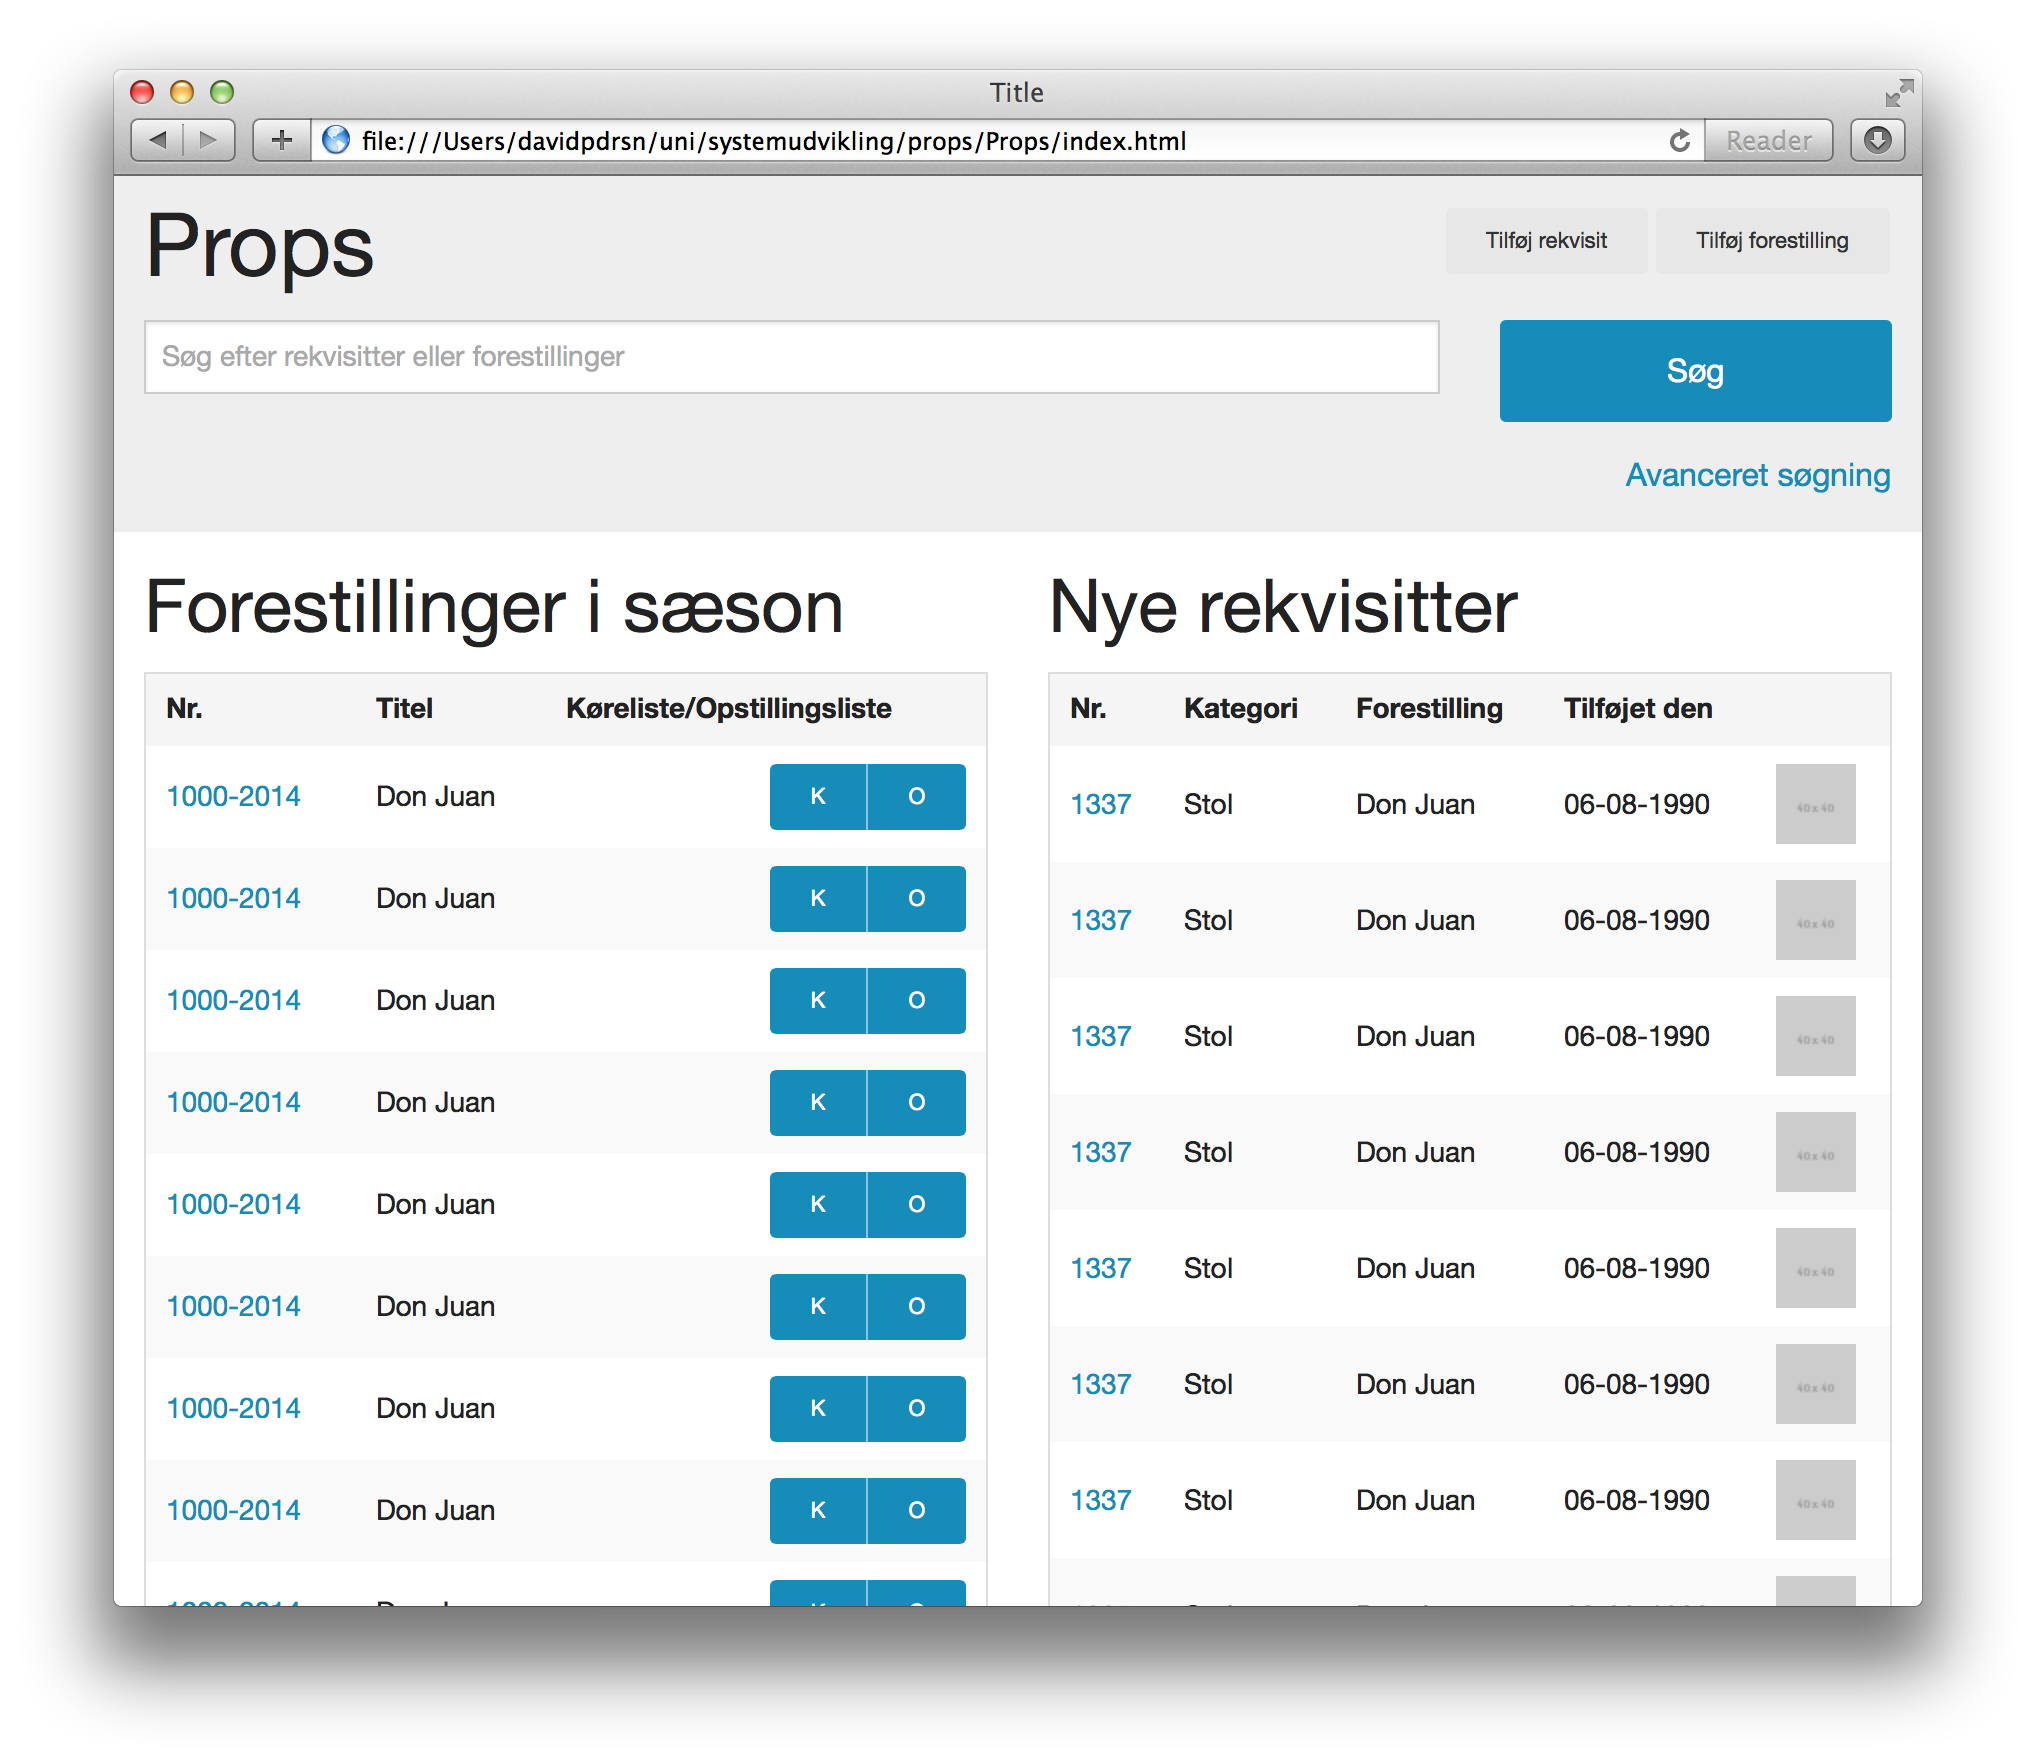
\includegraphics[scale=0.25]{prototype_frontpage.png}}
\newline
\textbf{Front page}\\
All pages will show a big search field up top as this is the primary feature of the site.\\
The frontpage also shows a list of productions that are being done this season as well as the latest props added to the database.
\newline
\newline
\centerline{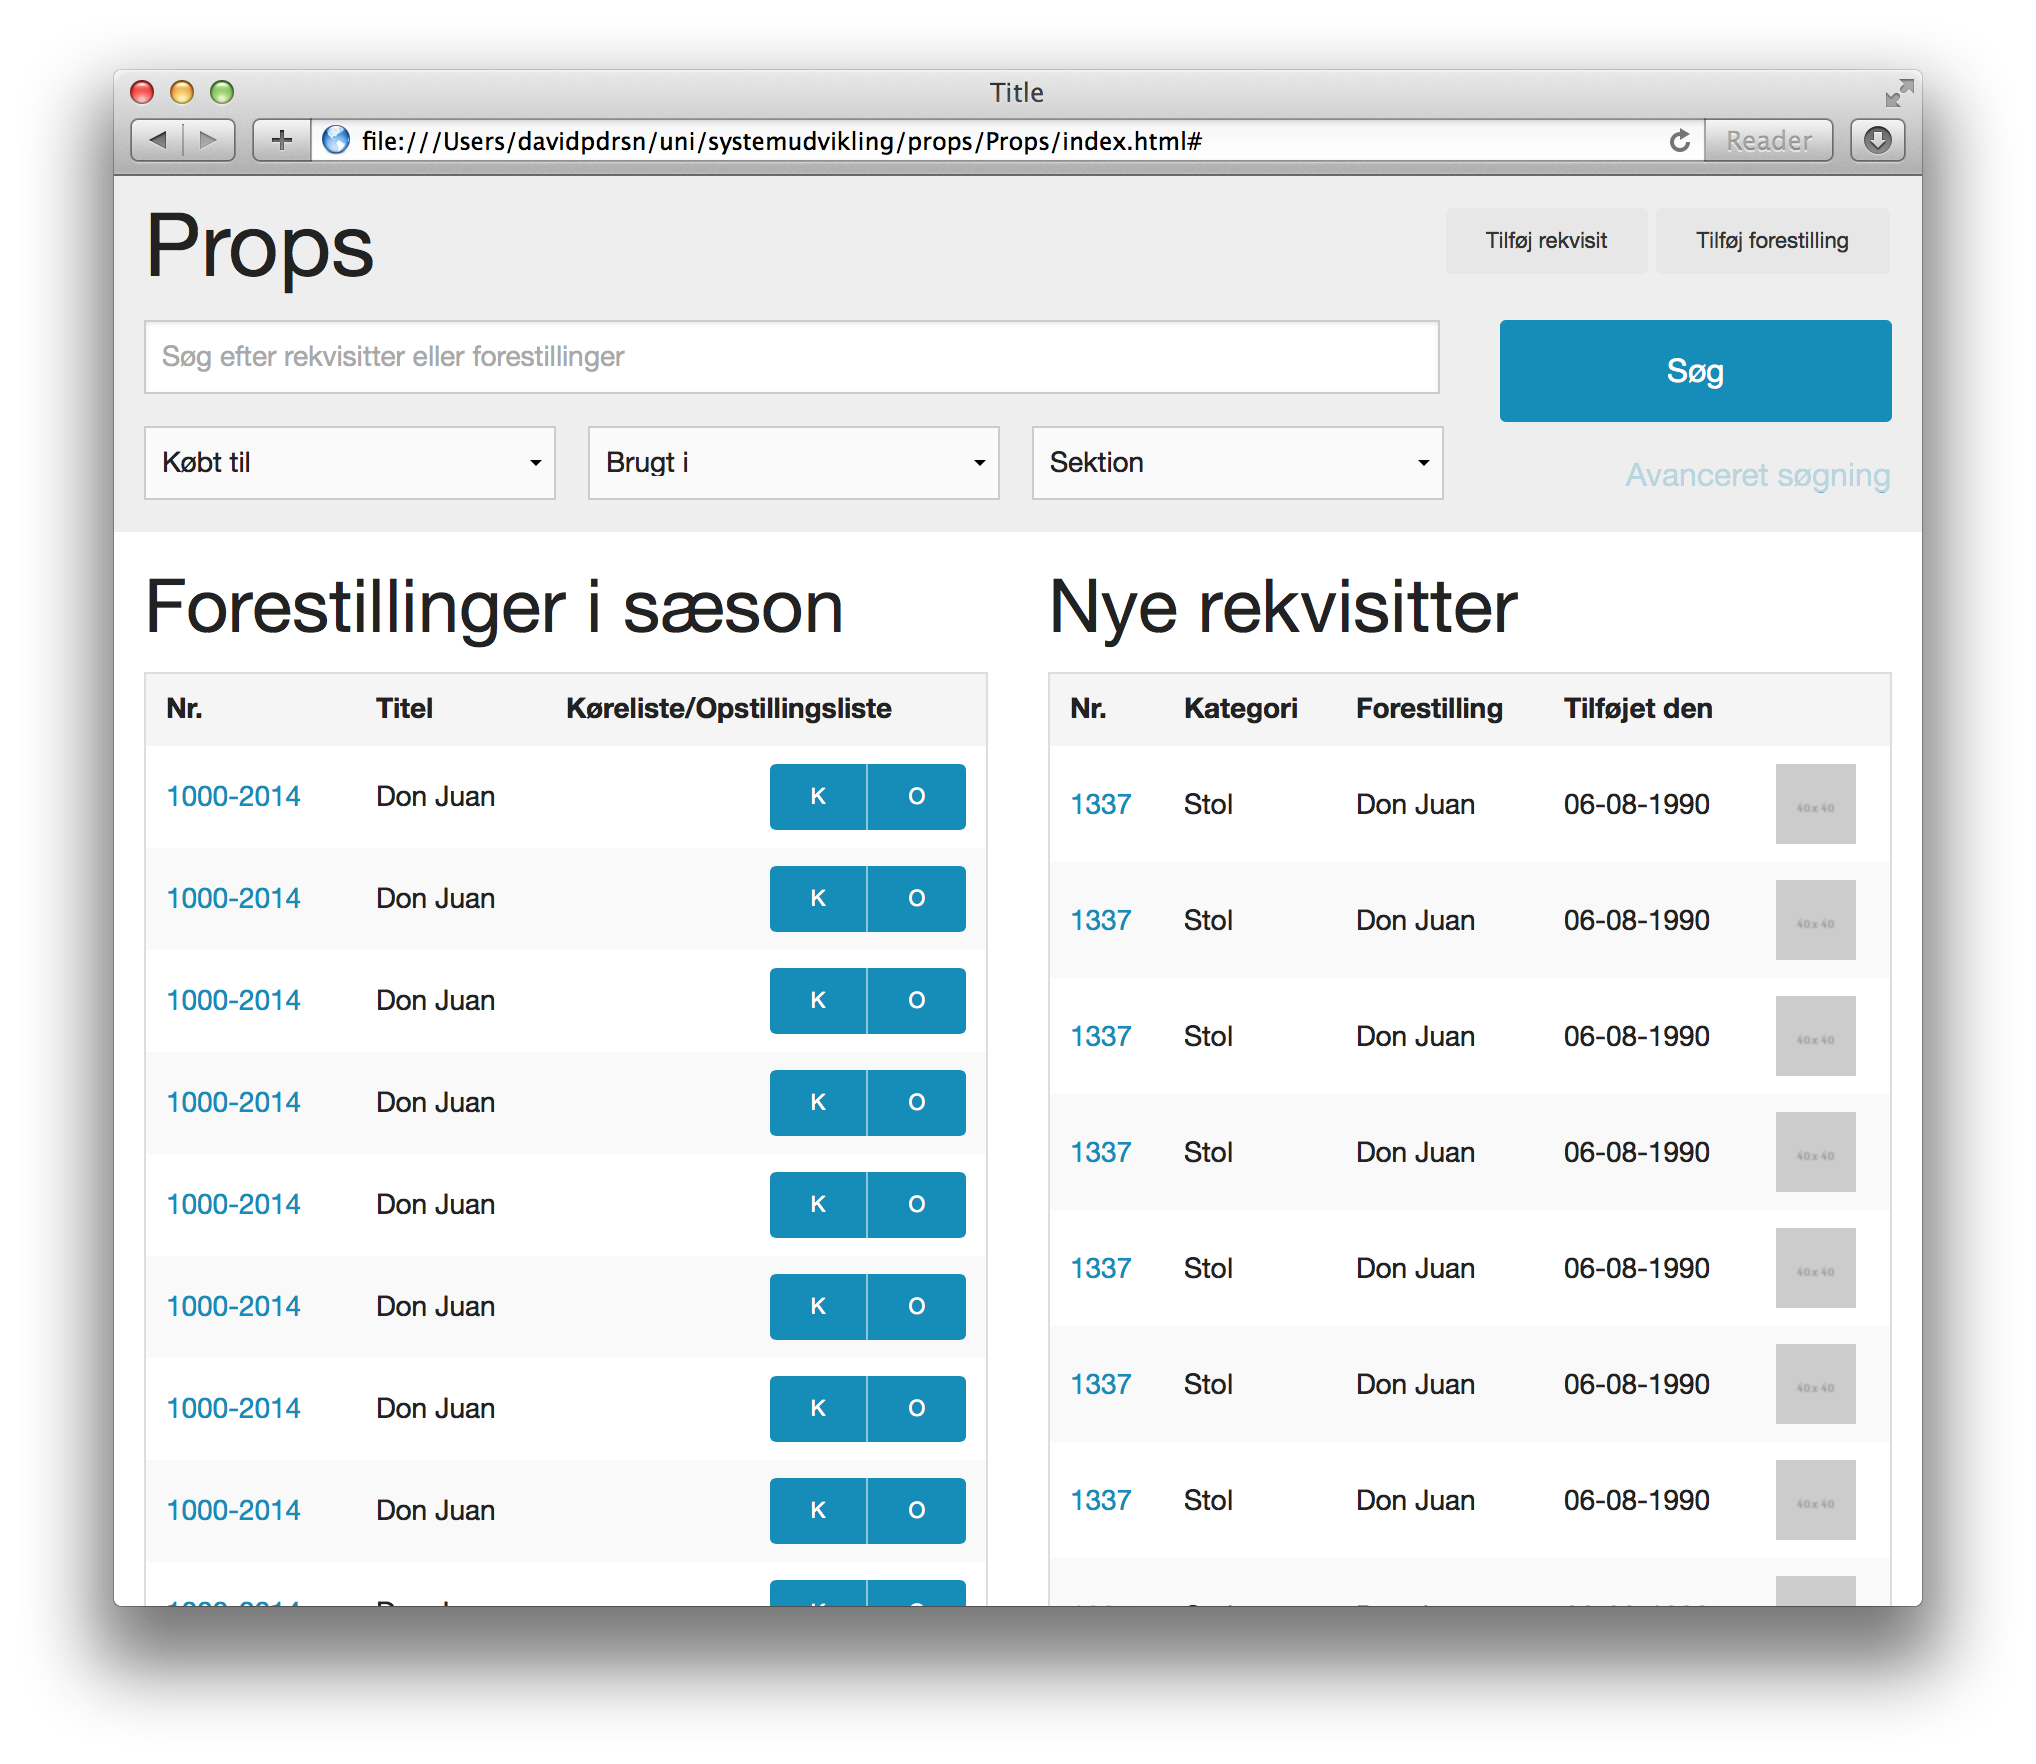
\includegraphics[scale=0.25]{prototype_advanced_search.png}}
\newline
\textbf{Front page with advanced search}\\
It is often useful to limit the scope of a search to a specfic production or a specific section of props. This can be done through some dropdown menus that appear when clicking on advanced search.
\newline
\newline
\centerline{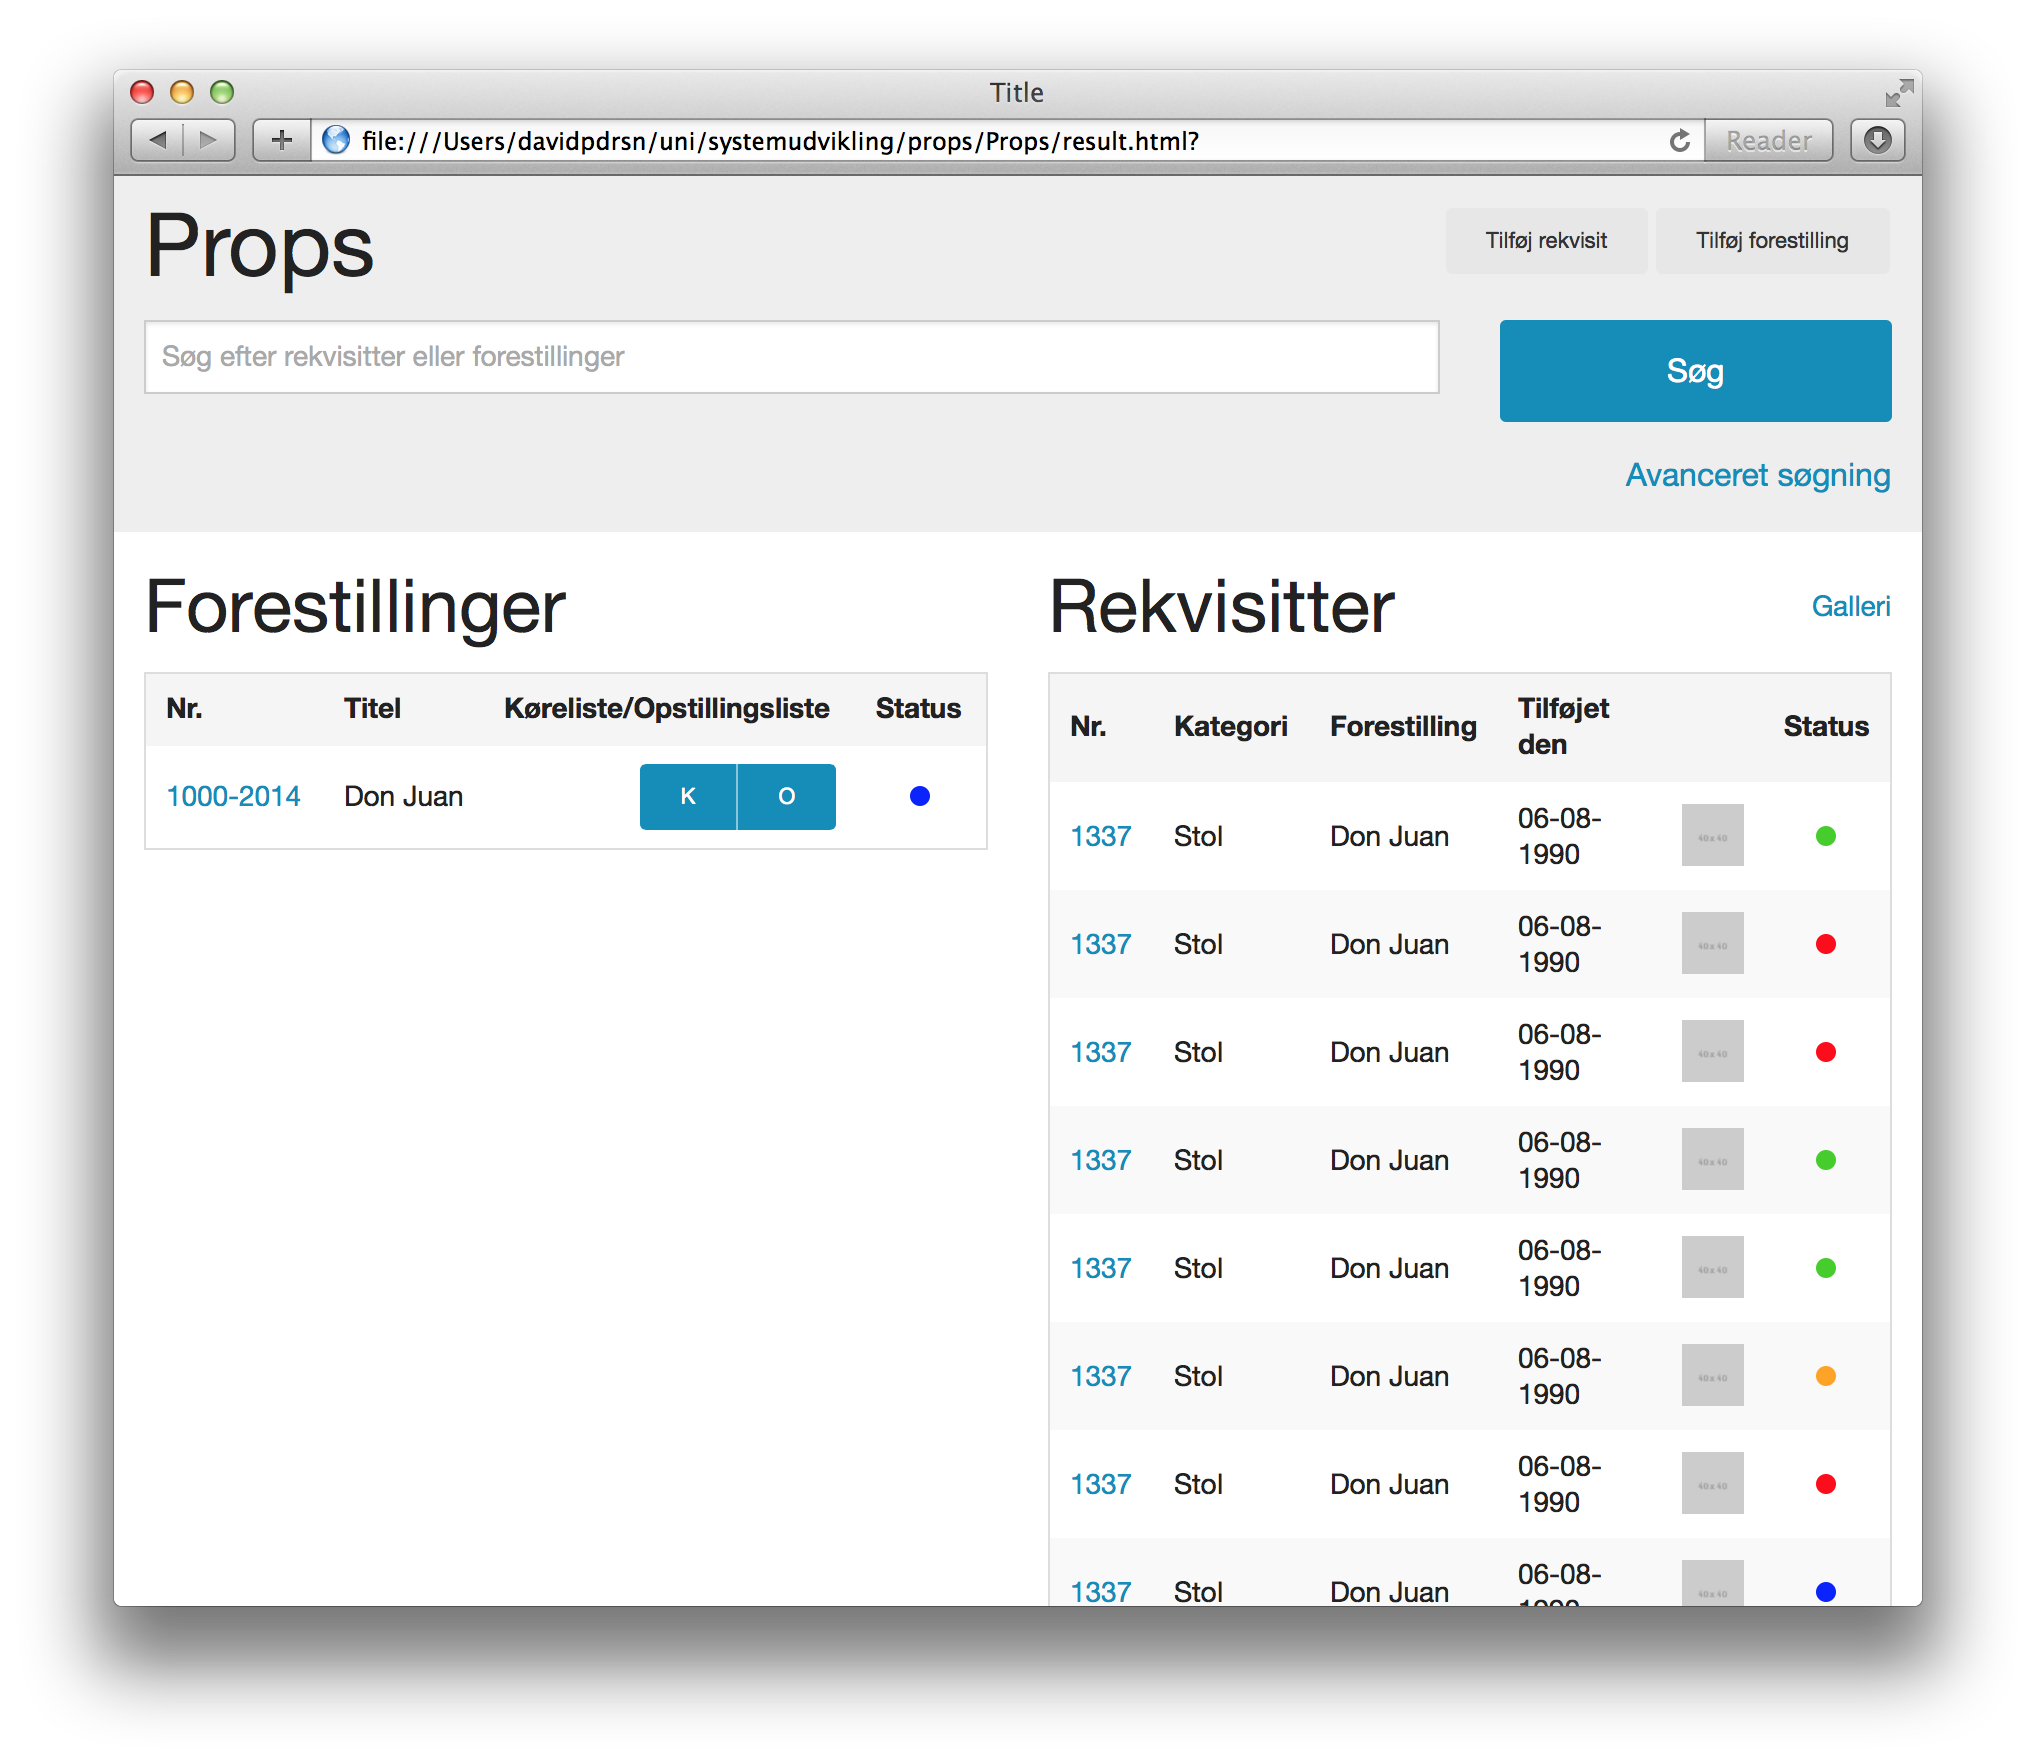
\includegraphics[scale=0.25]{prototype_search_result.png}}
\newline
\textbf{Search result page}\\
This page shows the result of doing a search. It shows the performances and props that were matched. Along with the attributes also shown on the frontpage it also shows the status of the prop and production. A status could be something like "reversed" or "free to use".
\newline
\newline
\centerline{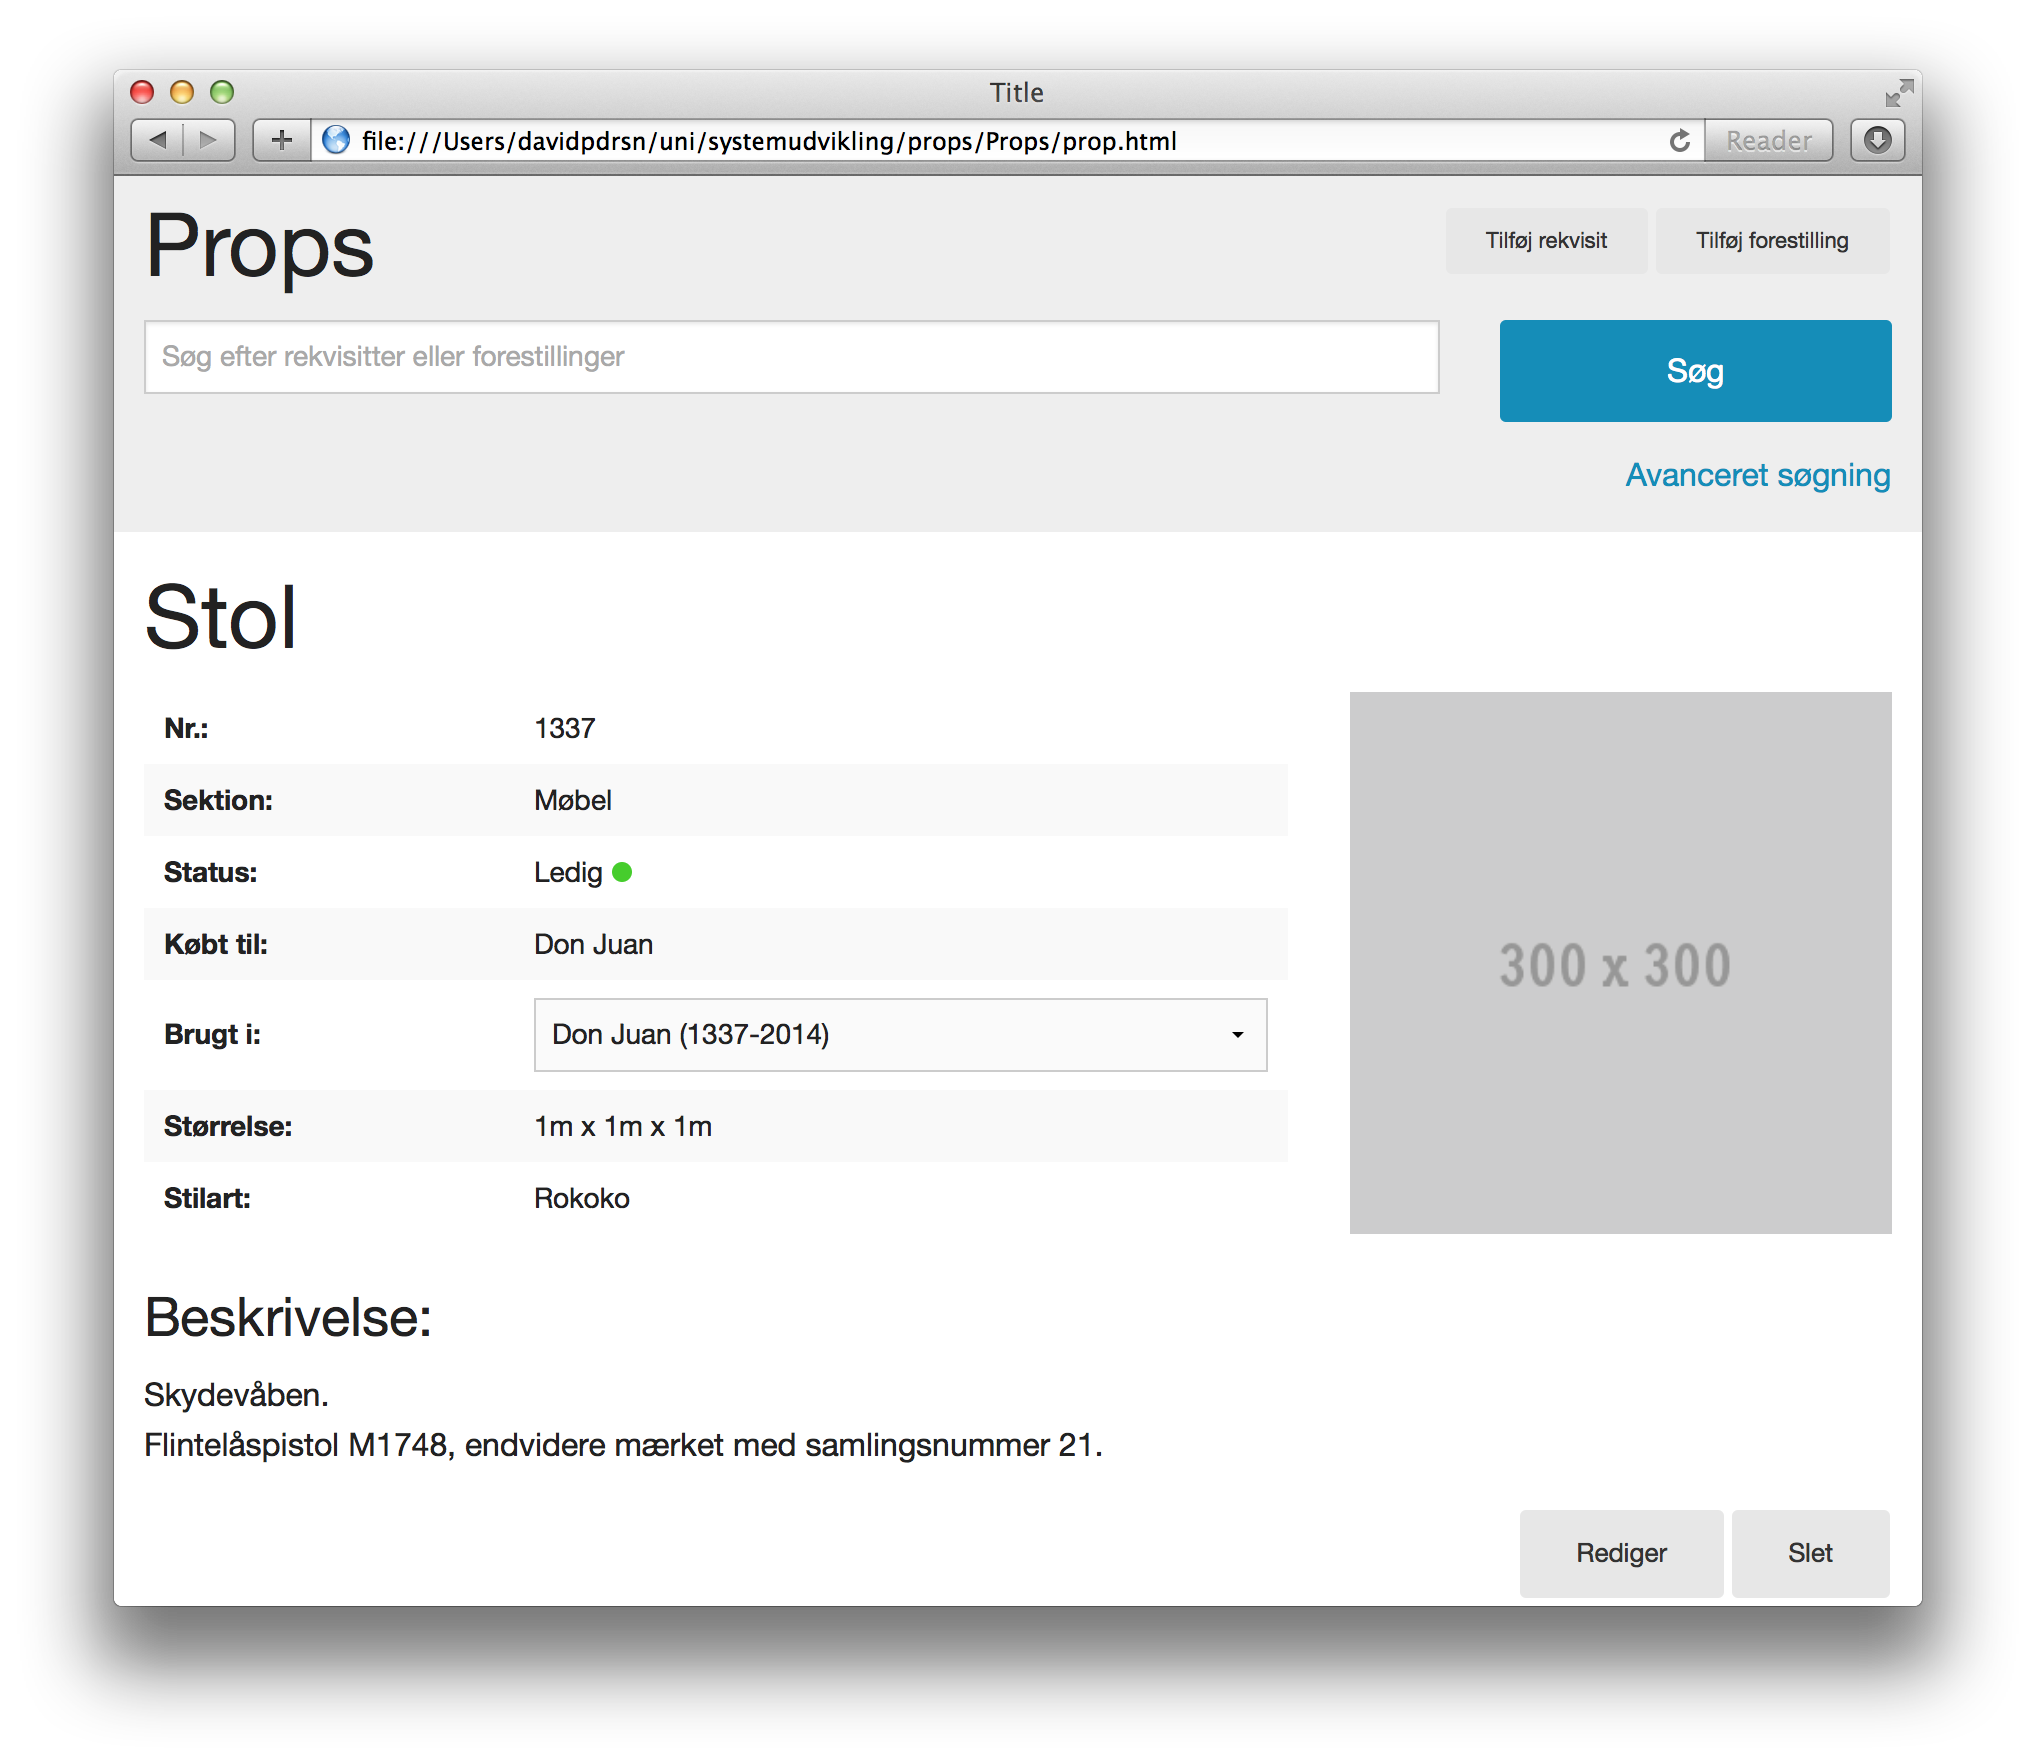
\includegraphics[scale=0.25]{prototype_show_prop.png}}
\newline
\textbf{Single prop page}\\
This is the page the shows information about a single prop in the database. It simply shows the attributes of the prop.
\subsection{b) Flow and user interactions}
Up until now we have been focusing on building backend functionality. This mean that at this point we don't yet have a user interface to give a demonstration of.
\subsection{c) Demo of prototype}
There is no actual behavior to give a demonstration of yet (see previous point).
\subsection{d) Review of latest think aloud test}
Since we handed in our last report we have not had any meetings with the client and have also not conducted any user tests. We also have no userinterface to test, yet.
\section{Version control}
We chose to use Git as our version control system. This gives us great confidence that we wont loose work and easy collaboration when using GitHub to host the repository.
\newline
\newline
We chose a simple and effective strategy for using version control. The master branch represents the project as it is right now. This means whats on the master branch should always be working and master is therefor not used when developing new features, fixing bugs, refactoring, etc. To do that we use topic branches and when they are in a finished state they get merged back into master and then deleted. This techniques works well because Git has such cheap branching and merging. This technique is also very easy to maintain because the number of concurrent branches are kept at a minimum.
\newline
\newline
See appendix A for our current commit log of the master branch. There is a total of 45 commits on topic branches not yet merged into master. They are not included in the log, since they might change.
\newline
\newline
Here is a short overview of the most important changes that has happended within the history of the application:
\begin{description}
  \item[Commit "d4b310e"] \hfill \\
    At this point the save method on our model class was feature complete. This method is really important since its an essential part of adding new records to the database. Since commit "d4b310e" we have started refactoring the method to make it more maintainable.
  \item[Commit "e4e1379"] \hfill \\
    From a testing perspecitive this commit is quite important. After this point the database will be automatically reset before every test. This ensures that tests that modify the database wont break other tests since the tests are ran in random order.
  \item[Commit "c72ba12"] \hfill \\
    This commit added a SQL file that can be used to build the database with the required schema.
  \item[Commit "e327b6a"] \hfill \\
    Up until this commit we had been working on some relatively low level infrastructure. This is the code that sits closest to the web browser and receives a representation of the request from the browser and finds out which code to run and which view to render. This is an essential part of our application flow as its part of every request.
\end{description}
See appendix B for important pieces of the application code.
\section{Project collaboration}
So far our collaboration with the client has been through planning meetings during the initial requirements elicitation phase. Here is a timeline of the meetings and participants:
\begin{description}
\item[March 13th]
  Mikkel Theut (chairman of the props department)
\item[March 20th]
  Martin Thaarup Larsen (head of the IT-department)
\item[March 25th]
  Mikkel Theut, Palle Henriksen (head of the furniture subdivision), Thomas Kolding (employed at the furniture subdivision)
\item[April 8th]
  Charlotte, Mikkel Theut, furniture subdivision
\item[April 9th]
  Mikkel Theut, Palle Henriksen, Thomas Kolding, Martin Thaarup Larsen, Claus Nepper Fakkenberg (employed at the props department and developer of the old system)
\end{description}
During each meeting we had allocated one person to taking notes and then later adding those notes to version control. This has been useful when preparing for other meetings and when writing the reports but other than that they have been used a lot.\\\\
We have not yet written any code documentation since we have not written any code.
\section{Appendices}
\subsection{Appendix A: Commit log}
\begin{verbatim}
commit 713e115b77ffb1b3d25d8880797059a1477809cc
Author: David Pedersen <dap@html24.net>
Date:   Thu May 8 17:12:54 2014 +0200

    add example setup

commit 39da04d6296b209999f24549a6e6a7c65bd556c0
Author: David Pedersen <dap@html24.net>
Date:   Thu May 8 16:41:32 2014 +0200

    extract instance vars method

commit 962e5f11e8ac29738bc3a29689e917ddd0d81033
Author: David Pedersen <dap@html24.net>
Date:   Thu May 8 16:32:06 2014 +0200

    extract update_sql and insert_sql methods

commit c8cb55ac699de3d8dd4eed46fc2c6e971a9cf6ce
Author: David Pedersen <dap@html24.net>
Date:   Thu May 8 16:28:53 2014 +0200

    extract new_record method

commit d4b310ea3b9fe13c34e0a6e0e82444fbad0a82e1
Author: David Pedersen <dap@html24.net>
Date:   Thu May 8 16:05:59 2014 +0200

    test that models that get saved gets timestamp

commit b714c289d2e6d08fdc1540570221f892c67a94c9
Author: David Pedersen <dap@html24.net>
Date:   Thu May 8 16:00:11 2014 +0200

    update things that depend on the the new database schema

commit 4772b5e418a8314931d7cc2f0fdc80063042651d
Author: Louise Knudsen <louise-w-knudsen@hotmail.com>
Date:   Thu May 8 15:25:52 2014 +0200

    save() auto date added

commit 2ebf609173b27f913f3a9fd362c559c9dc168da9
Merge: 06296c0 28af238
Author: Bach <helenafbach@hotmail.com>
Date:   Thu May 8 15:10:17 2014 +0200

    Merge branch 'master' of https://github.com/Project-Props/Props

commit 06296c06b5e9ac02362222314eb99476f00bf780
Author: Bach <helenafbach@hotmail.com>
Date:   Thu May 8 15:06:55 2014 +0200

    Users table deleted and added category- and subcategory attributes in props table

commit 28af238d7dc3ed0a517233ad93ca6cddca97a431
Author: David Pedersen <dap@html24.net>
Date:   Thu May 8 14:58:24 2014 +0200

    extract default title into variable so its not duplicated

commit 9a102686ed1329d7e0a402523db8fd9ba524100f
Merge: 8790140 41492db
Author: Bach <helenafbach@hotmail.com>
Date:   Thu May 8 14:40:33 2014 +0200

    Merge branch 'master' of https://github.com/Project-Props/Props

commit 879014014c4496b52ddd85b1a314218d1705db94
Author: Bach <helenafbach@hotmail.com>
Date:   Thu May 8 14:40:11 2014 +0200

    method call in header

commit 7f83a26d4913b3d2327121db0b89dc42e2eddf26
Author: Bach <helenafbach@hotmail.com>
Date:   Thu May 8 14:31:02 2014 +0200

    title variable created

commit 41492db1e5ca9527ad14d0a6ef4620ed6086200a
Author: David Pedersen <dap@html24.net>
Date:   Thu May 8 14:30:55 2014 +0200

    add todo

commit 510d06f082fb2d256abdd39a0685c6e90e7c65af
Author: David Pedersen <david.pdrsn@gmail.com>
Date:   Sun May 4 17:03:00 2014 +0200

    add some todo notes

commit 737702bf67aeb1cc857592b2d56972fca2d7d867
Author: David Pedersen <david.pdrsn@gmail.com>
Date:   Sun May 4 16:59:55 2014 +0200

    fix bug in Request#param

commit edf70dbbd244917e5072bff8b8a03780ed1b72d6
Author: David Pedersen <david.pdrsn@gmail.com>
Date:   Sun May 4 16:53:49 2014 +0200

    remove logging from database class

commit 05456c3d80b5cf3514f65241af7269db95a212fc
Author: David Pedersen <david.pdrsn@gmail.com>
Date:   Sun May 4 16:53:22 2014 +0200

    add delete method to Prop and add Section model

commit 2ebffe53fc911068f7d4b301ce6bee280f471420
Author: David Pedersen <david.pdrsn@gmail.com>
Date:   Sun May 4 16:52:37 2014 +0200

    update Request#param to convert bools and numbers to actual types

commit 2b892cf28cf4baa733eac98206a51f5e4b6735a9
Author: David Pedersen <david.pdrsn@gmail.com>
Date:   Sun May 4 16:52:11 2014 +0200

    remove logger

commit 8c55b46953bb960cb8bec4e9d4f97434d8eff9d2
Author: David Pedersen <david.pdrsn@gmail.com>
Date:   Sun May 4 16:49:03 2014 +0200

    add default scope to Model#all

commit aaecad0bcf2ea6c1198caae441cf7c62a10138fa
Author: David Pedersen <david.pdrsn@gmail.com>
Date:   Sun May 4 16:48:23 2014 +0200

    update Router#define_route to accept both a method path and callable

commit a76d93c86f05d6551817460ebb3f1d47573ea598
Merge: 3547f11 4eff41a
Author: David Pedersen <david.pdrsn@gmail.com>
Date:   Sun May 4 15:40:58 2014 +0200

    Merge branch 'model_save' into davids-test-branch

commit 4eff41a00dfb1042d444780765dfc612dd8157cb
Author: David Pedersen <david.pdrsn@gmail.com>
Date:   Sun May 4 15:40:01 2014 +0200

    add note about duplication

commit 5ec8a1810222af5b5221b82e97e1ed5bd5755fd0
Author: David Pedersen <david.pdrsn@gmail.com>
Date:   Sun May 4 15:37:09 2014 +0200

    load files a little smarter

commit 3737aeb18213f41ac19de88eb18d77348fddad92
Author: David Pedersen <david.pdrsn@gmail.com>
Date:   Sun May 4 15:28:24 2014 +0200

    misc whitespace

commit b170dbf121ce8154141439d441e82cfe3e700f99
Author: David Pedersen <david.pdrsn@gmail.com>
Date:   Sun May 4 15:23:00 2014 +0200

    refactor Model::find a little

commit 3c4741b17d634e4104f3abb90e2ebae2add39121
Author: David Pedersen <david.pdrsn@gmail.com>
Date:   Sun May 4 14:57:47 2014 +0200

    find array of related objects through join table

commit 43b992e65d074baaf6cd7cfe2c79843911b9a62b
Author: David Pedersen <david.pdrsn@gmail.com>
Date:   Sun May 4 14:24:52 2014 +0200

    update name of test

commit 8e6fa22f6e564d83501df680442e4b6035468fc0
Author: David Pedersen <david.pdrsn@gmail.com>
Date:   Fri May 2 22:24:10 2014 +0200

    make Model#database_connection() method protected

commit 2c92ffccf290086e3201c4c1fd4299b64c692c48
Author: David Pedersen <david.pdrsn@gmail.com>
Date:   Fri May 2 22:11:07 2014 +0200

    move commas to infront

commit 0d3a1b1c522ad1c1522fe69c6e989329f01f77a0
Author: David Pedersen <david.pdrsn@gmail.com>
Date:   Fri May 2 22:07:41 2014 +0200

    handle the fact that productions cannot autogenerate their own IDs

commit 10f3bdc1c50c55d8123780ca6fd5a26ed81a9565
Author: David Pedersen <david.pdrsn@gmail.com>
Date:   Fri May 2 21:44:46 2014 +0200

    log when performing an sql query

commit 6ef9914e618fe5c60cb02d2755521a8988478e1d
Author: David Pedersen <david.pdrsn@gmail.com>
Date:   Fri May 2 21:44:26 2014 +0200

    create log file if it doesn't exist

commit 6e9e2f7dcc0c36d096950b7061d8b8cc04daf4f0
Author: David Pedersen <david.pdrsn@gmail.com>
Date:   Fri May 2 21:43:50 2014 +0200

    remove log from git repo

commit 4c26a139e19cbb46464e7fb2daf79c25b93f26a4
Author: David Pedersen <david.pdrsn@gmail.com>
Date:   Fri May 2 21:39:46 2014 +0200

    add monolog, wrapper class, and log file

commit 1ccfb4190898108b0f68ede2ca0bfe7b9bfd2a7f
Author: David Pedersen <david.pdrsn@gmail.com>
Date:   Fri May 2 21:39:18 2014 +0200

    require all files in lib before running tests

commit 2b0220e4cc2d74bca9ae744e80c315a28d3583bc
Author: David Pedersen <david.pdrsn@gmail.com>
Date:   Fri May 2 21:38:58 2014 +0200

    require all files dynamically in all.php

commit 78dbfb9f2bd3551d9455229176b0d701c3a02526
Author: David Pedersen <david.pdrsn@gmail.com>
Date:   Fri May 2 20:48:54 2014 +0200

    make next_insert_id() protected so subclasses can override it
    
    This would be the case for Production since it handles IDs a little
    differently

commit 2aabcf3a1cbe9a849dbe42ea441d6de24cbfaff9
Author: David Pedersen <david.pdrsn@gmail.com>
Date:   Fri May 2 20:47:24 2014 +0200

    uppercase some sql

commit 265ff35b333310f67f0117cb10e7a61d84ec9321
Author: David Pedersen <david.pdrsn@gmail.com>
Date:   Fri May 2 20:45:43 2014 +0200

    make Database#query throw an exception if the query is not valid

commit 4e4cca375994137474ef1f5ca3a1652cc08ed979
Author: David Pedersen <david.pdrsn@gmail.com>
Date:   Fri May 2 20:32:09 2014 +0200

    improve tests for Model#save and fix bugs related to generatings IDs
    
    There were several problems with the old code
    
    - In our test case mysql_insert_id() returned zero for some reason and
      the record wasn't found when you tried to find it with Model::find.
      This was fixed by doing some SQL to manually retrieve the last ID
      inserted and just increment it.
    
    I also added some more assertions to the save test to have a little more
    confidence that it actually was working correctly.

commit 706c78ec79c3986ea876a9610e22184e52b1622a
Author: David Pedersen <david.pdrsn@gmail.com>
Date:   Fri May 2 20:17:46 2014 +0200

    update Model::find to handle cases when $id is 0
    
    Only the case where $id was set to NULL was being tested. And in the
    code the condition of the if statement was simply if ($id) { ... }.
    
    However in PHP 0 is a falsy value (evaluate to false in an if statment)
    so it wouldn't actually search for a record that had it 0.
    
    This was
    fixed using is_null in the condition instead.

commit 3547f11caff26c8309bfb4c1e4ebb1e01348f21e
Author: David Pedersen <david.pdrsn@gmail.com>
Date:   Fri May 2 20:08:40 2014 +0200

    link to normalize.css and jquery
    
    normalize.css is small css stylesheet that some smart people have
    written. It will normalize the way a lot of standard browser elements
    look on different browsers. This makes it easier to style them since you
    have a uniform base.
    
    jQuery is a javascript library that makes it easier to do all sorts of
    common things.
    
    We are for sure gonna need these two things at some point down the road.

commit 9fa50894e575416a480bd6ac55fecb4c03612260
Author: David Pedersen <david.pdrsn@gmail.com>
Date:   Fri May 2 20:04:35 2014 +0200

    make sample feature test not fail

commit d72f4a5f4277f2ef7ee0738d0d3859294414f199
Author: David Pedersen <david.pdrsn@gmail.com>
Date:   Fri May 2 11:06:18 2014 +0200

    remove unused constants

commit a3ea9ccab39c442f99ef386edb47ee2a26384e7b
Author: David Pedersen <david.pdrsn@gmail.com>
Date:   Thu May 1 21:57:20 2014 +0200

    refactor __call in model making it more clear

commit 02a06c6f3046ebd2d1d8a16ba11412550c93dbce
Author: David Pedersen <david.pdrsn@gmail.com>
Date:   Thu May 1 21:57:09 2014 +0200

    use database class in model

commit 38384467635f5451acad5e5fc6b067dd0742f3cf
Author: David Pedersen <david.pdrsn@gmail.com>
Date:   Thu May 1 21:39:28 2014 +0200

    make use of Database class in test listener

commit b12d1265e9a71286aef32c9d0d77d5d6e63d87fe
Author: David Pedersen <david.pdrsn@gmail.com>
Date:   Thu May 1 21:38:36 2014 +0200

    add Database class and other related classes

commit eaf15f22add6a0a36da74d6b11a8273a523114a6
Author: David Pedersen <david.pdrsn@gmail.com>
Date:   Thu May 1 10:16:00 2014 +0200

    make has_one return an empty array by default
    
    otherwise there will be errors when calling methods that don't exist

commit 4ea5da40ab615dab05a0d2db1272bbb9211f0f88
Author: David Pedersen <david.pdrsn@gmail.com>
Date:   Thu May 1 10:06:06 2014 +0200

    use Quoter class to remove some conditionals

commit 6bacb96efffa6712710d0c647e7962185668a97c
Author: David Pedersen <david.pdrsn@gmail.com>
Date:   Thu May 1 09:50:51 2014 +0200

    remove some trailing whitespace

commit 76a951694c5ebcde937fd2d9ba28fd3fe0f184ba
Author: David Pedersen <david.pdrsn@gmail.com>
Date:   Wed Apr 30 22:12:57 2014 +0200

    add quoter class

commit 3782410eba3b449d0e6637f2b20d9a8bb7b2e623
Author: David Pedersen <david.pdrsn@gmail.com>
Date:   Wed Apr 30 21:58:45 2014 +0200

    add test for Model::find when ID is null

commit a113adcf3ba1f09bdb35202da3a6b2ccb19972bc
Author: David Pedersen <david.pdrsn@gmail.com>
Date:   Wed Apr 30 21:57:10 2014 +0200

    reorder some tests

commit 2d3f34564ea12681591663e6b5ecc8105aad69eb
Author: David Pedersen <david.pdrsn@gmail.com>
Date:   Wed Apr 30 21:56:18 2014 +0200

    reorder methods

commit 5662f5548019556bcc44f4a31f782d405e1dc3cb
Author: David Pedersen <david.pdrsn@gmail.com>
Date:   Wed Apr 30 21:54:39 2014 +0200

    add back methods in model that had disappeared for some reason

commit 52bbf8a8d3fe2f0b769da66c43808a871f763440
Author: David Pedersen <david.pdrsn@gmail.com>
Date:   Wed Apr 30 21:32:00 2014 +0200

    remove some trailing whitespace

commit 5953009304f1a29a5cd884adf96535eb87ba915f
Author: David Pedersen <david.pdrsn@gmail.com>
Date:   Wed Apr 30 21:30:02 2014 +0200

    make __call in Model public

commit 9400cfcb1afd05ff013cc8c2cd5820b3ce848fc2
Author: David Pedersen <david.pdrsn@gmail.com>
Date:   Wed Apr 30 21:29:24 2014 +0200

    uncomment commented out tests

commit 5c32ef71b2e9a5363d772dcc4aed4850708da5b0
Author: David Pedersen <david.pdrsn@gmail.com>
Date:   Wed Apr 30 21:29:21 2014 +0200

    remove var_dump

commit 99fde53284fac6609ac4a63047315367ab66cb9f
Author: Louise Knudsen <louise-w-knudsen@hotmail.com>
Date:   Wed Apr 30 17:25:06 2014 +0200

    fixed not nummeric value i quotes in save()

commit cda259daf1020a8dd79384c0e97b28115f680443
Author: Louise Knudsen <louise-w-knudsen@hotmail.com>
Date:   Wed Apr 30 16:44:00 2014 +0200

    fixed rebase bug in find

commit 4c431bc74168029e29bd3db5980f0500c69799f5
Author: Louise Knudsen <louise-w-knudsen@hotmail.com>
Date:   Wed Apr 30 16:28:14 2014 +0200

    if statement in find added, save() for new records done

commit aa144dd2b997c5c3951ddbc96f5eaf2344505f9a
Author: Louise Knudsen <louise-w-knudsen@hotmail.com>
Date:   Wed Apr 30 13:02:59 2014 +0200

    update part of save done

commit 18fcc1ad8bcff29ac30043b958961e0e9e894110
Author: David Pedersen <david.pdrsn@gmail.com>
Date:   Thu May 1 20:45:30 2014 +0200

    only reset the database before every test and when the entire suite is
    done

commit 41f9c9a2c9037e739c2643f7d26e6cb35e7f73a8
Author: David Pedersen <david.pdrsn@gmail.com>
Date:   Thu May 1 20:38:36 2014 +0200

    add some documatation for controller, router, and view

commit f0e5bc7d106010f6abbb1ea374397ea576156ef5
Author: David Pedersen <david.pdrsn@gmail.com>
Date:   Wed Apr 30 15:31:48 2014 +0200

    remove trailing whitespace

commit a6bcc18b8689ee97ede28eb92212dfc10e2ea33d
Author: David Pedersen <david.pdrsn@gmail.com>
Date:   Wed Apr 30 15:30:03 2014 +0200

    add dynamic association finding methods

commit 418f788deb433a5e24c2f2bbae64f0341d8d9801
Author: David Pedersen <david.pdrsn@gmail.com>
Date:   Wed Apr 30 15:29:02 2014 +0200

    expand find to work with ids that are strings

commit e4e1379f6deaed9665fca84b1ce2e76c22292a84
Author: David Pedersen <david.pdrsn@gmail.com>
Date:   Wed Apr 30 12:07:06 2014 +0200

    reset the database before and after every test

commit 11355f607b73d4d05d13c84e13d71b9051180321
Author: David Pedersen <david.pdrsn@gmail.com>
Date:   Wed Apr 30 11:04:34 2014 +0200

    throw exception when find is called with non-existing id

commit 27456bea631e33fa2a6b8c268f74b2a335eeb04c
Author: David Pedersen <david.pdrsn@gmail.com>
Date:   Wed Apr 30 10:54:13 2014 +0200

    add Model::all()

commit ba2507c236654536965c88aad5380035f5b32668
Author: David Pedersen <david.pdrsn@gmail.com>
Date:   Wed Apr 30 10:33:00 2014 +0200

    remove empty methods

commit 5225d7cb08178e5ddfd7167495fd0a360c308ab6
Author: David Pedersen <david.pdrsn@gmail.com>
Date:   Wed Apr 30 10:19:47 2014 +0200

    break up long line

commit 3e4efc7820e7626f62009d74e759602637519f9b
Author: David Pedersen <david.pdrsn@gmail.com>
Date:   Wed Apr 30 10:19:13 2014 +0200

    remove evil try catch

commit bb1d4f97fb0ba8b991a4f88ea756c3cd1ed7cf10
Author: David Pedersen <david.pdrsn@gmail.com>
Date:   Tue Apr 29 17:36:12 2014 +0200

    update script for running all tests to use new config

commit 963fc40e074e55afa500017480c2c68e923785dd
Author: David Pedersen <david.pdrsn@gmail.com>
Date:   Tue Apr 29 17:36:06 2014 +0200

    update phpunit config

commit ee368d1a714b9a8093e299d89f06477ff270e595
Author: David Pedersen <david.pdrsn@gmail.com>
Date:   Tue Apr 29 17:35:29 2014 +0200

    replace self with static, fixes #12

commit 99563527009a901063a609da63d85684a9471320
Author: David Pedersen <david.pdrsn@gmail.com>
Date:   Mon Apr 28 22:05:49 2014 +0200

    add extra assertion in model test, just to be sure

commit 537e52024b31ef76aa2aad6e6ab19dfccd93a395
Author: David Pedersen <david.pdrsn@gmail.com>
Date:   Mon Apr 28 17:55:28 2014 +0200

    setup phpunit to always show errors

commit 87421699342d687c8a0faa16e7c264dc3af898f2
Author: David Pedersen <david.pdrsn@gmail.com>
Date:   Mon Apr 28 17:47:05 2014 +0200

    put database related values into constants

commit e38c64bad0c90c7954782acad5b526305b0bf16f
Author: David Pedersen <david.pdrsn@gmail.com>
Date:   Mon Apr 28 17:45:23 2014 +0200

    cache connection in model class

commit 1765529b47fba95ce1692d93c597aea42a418c3f
Author: Louise Knudsen <louise-w-knudsen@hotmail.com>
Date:   Mon Apr 28 17:38:40 2014 +0200

    models folder added, prop class added

commit c56540bc7419154cbd56dcbba2e5722ceccf0edd
Author: David Pedersen <david.pdrsn@gmail.com>
Date:   Mon Apr 28 17:28:31 2014 +0200

    update formatting of whitespace

commit 542c4e51c643ba144da3443cde3550eea2658870
Author: David Pedersen <david.pdrsn@gmail.com>
Date:   Mon Apr 28 17:28:29 2014 +0200

    up

commit 247759978ecaa0e1136159bfaae0448d0ad9fefc
Author: Louise Knudsen <louise-w-knudsen@hotmail.com>
Date:   Mon Apr 28 17:18:51 2014 +0200

    find() added to Model class

commit 1682b773eb22608aea59fe5d1db725315580622b
Merge: bea1323 ddfaef3
Author: David Pedersen <david.pdrsn@gmail.com>
Date:   Mon Apr 28 14:22:53 2014 +0200

    Merge pull request #5 from Project-Props/setup-css-and-js
    
    Setup css and js

commit ddfaef30a62529359a161b1a6d21dd773c949f19
Author: David Pedersen <david.pdrsn@gmail.com>
Date:   Mon Apr 28 14:05:53 2014 +0200

    remove undefined variables

commit e17b72d681b72963a130876bd85b44b734babf09
Author: David Pedersen <david.pdrsn@gmail.com>
Date:   Mon Apr 28 14:05:43 2014 +0200

    add css file and javascript file

commit 8c8781ff973dc00d4e5e0295f1d10be3bb5d873f
Author: David Pedersen <david.pdrsn@gmail.com>
Date:   Mon Apr 28 14:05:32 2014 +0200

    add HTML boilerplate to layout

commit 88b7b9459484893ac5736151e55251d7ec9054ca
Author: David Pedersen <david.pdrsn@gmail.com>
Date:   Mon Apr 28 14:05:04 2014 +0200

    always include views from "views" folder

commit bea132342ebdb06c27408a71850cd498e411a052
Merge: 1959cb7 eb48105
Author: David Pedersen <david.pdrsn@gmail.com>
Date:   Mon Apr 28 13:43:57 2014 +0200

    Merge branch 'tests-and-phpdoc'

commit eb48105fb252bbd1d50751326e375b113543b0d1
Author: Bach <helenafbach@hotmail.com>
Date:   Mon Apr 28 13:43:06 2014 +0200

    install dependencies

commit 43c5b05723bfb8455dfedad6a4a8648cff4fba64
Author: David Pedersen <david.pdrsn@gmail.com>
Date:   Mon Apr 28 13:13:51 2014 +0200

    install dependencies

commit dc2926721442781c4f511de76032a916e5eb3ef4
Author: Bach <helenafbach@hotmail.com>
Date:   Mon Apr 28 13:10:21 2014 +0200

    add missing emails

commit 1959cb7bd7d691947655dd0fdcfc941be23fdfb9
Merge: 48ef399 683deaa
Author: weesgaard <louise-w-knudsen@hotmail.com>
Date:   Mon Apr 28 12:08:26 2014 +0200

    Merge pull request #2 from Project-Props/render-layout
    
    Reduce HTML duplication by introducing a layout

commit 48ef399b1883f7e5f40607a7988fb267364257a8
Merge: 42ac8ab 8635c44
Author: weesgaard <louise-w-knudsen@hotmail.com>
Date:   Mon Apr 28 11:49:04 2014 +0200

    Merge pull request #4 from Project-Props/create_database
    
    Create database

commit b3030bd82d7a18b85c63cd386004068b7c9832ef
Author: David Pedersen <david.pdrsn@gmail.com>
Date:   Mon Apr 28 11:44:43 2014 +0200

    add bootstrap script

commit 8635c4483d0b5f74c029b2e08e91019326000a27
Author: Louise Knudsen <louise-w-knudsen@hotmail.com>
Date:   Mon Apr 28 11:39:49 2014 +0200

    tests fixed

commit 66e5bcfd67b7053296a788a6e44bc223df0da87a
Author: David Pedersen <david.pdrsn@gmail.com>
Date:   Mon Apr 28 11:25:46 2014 +0200

    add script for running all tests

commit bac434fddaec756d421823ab82d7e6b385d3f7da
Author: Louise Knudsen <louise-w-knudsen@hotmail.com>
Date:   Mon Apr 28 11:23:05 2014 +0200

    test added, commets on database-script added

commit bdbeff08a4f0dcc93c1672ac98da1218a0b1f086
Author: David Pedersen <david.pdrsn@gmail.com>
Date:   Mon Apr 28 11:19:40 2014 +0200

    update readme

commit f34fbfdbbc5e8e4545d4e7e43d21f3888dc77cc3
Author: David Pedersen <david.pdrsn@gmail.com>
Date:   Mon Apr 28 11:12:22 2014 +0200

    Write about feature tests in readme

commit 09dfb08792df56c67cbf77238b66907ccbfd2d41
Author: David Pedersen <david.pdrsn@gmail.com>
Date:   Mon Apr 28 11:08:17 2014 +0200

    make sample behat config

commit 459525eca0726923cb2361d0fabda3eaf1ffad57
Author: David Pedersen <david.pdrsn@gmail.com>
Date:   Mon Apr 28 11:00:27 2014 +0200

    initialize behat and add a sample test

commit c72ba126936e8ae7d780519356691637c6f164b2
Merge: 7619352 cae0f3d
Author: Bach <helenafbach@hotmail.com>
Date:   Mon Apr 28 10:55:55 2014 +0200

    Merge branch 'create_database' of https://github.com/Project-Props/Props into create_database

commit 7619352db84a755574b0b67f7ad36d1d27f81941
Author: Bach <helenafbach@hotmail.com>
Date:   Mon Apr 28 10:54:48 2014 +0200

    added 'use - statement and changed the order of the props- and productions tables

commit cae0f3ddd14ad55d6b6950e9fb797faf5a3e028d
Author: Louise Knudsen <louise-w-knudsen@hotmail.com>
Date:   Mon Apr 28 10:53:46 2014 +0200

    props test added

commit 78cf60afbafa4e7bebb490b58b82f0caa8f7781d
Author: David Pedersen <david.pdrsn@gmail.com>
Date:   Mon Apr 28 10:46:38 2014 +0200

    add BDD testing frameworks

commit 683deaa0c0034368064e1bae0c63b4afdc16b189
Author: David Pedersen <david.pdrsn@gmail.com>
Date:   Sun Apr 27 09:46:22 2014 +0200

    make View#render_template private

commit 0690197c2019f6749cdb2c198365ee75a39814ed
Author: David Pedersen <david.pdrsn@gmail.com>
Date:   Sun Apr 27 09:39:13 2014 +0200

    Make View#render render a layout which then renders the template

commit c6ac01df1d11d045b16d5bdf59110ff74f010c25
Author: David Pedersen <david.pdrsn@gmail.com>
Date:   Sun Apr 27 09:33:29 2014 +0200

    Make env parameter optional to View#render method
    
    Sometimes it might not be necessary to specify one

commit cbee1135eac3bb9130139511c4e8868e5ed2a338
Author: David Pedersen <david.pdrsn@gmail.com>
Date:   Sun Apr 27 09:28:53 2014 +0200

    rename Request#uri method to url

commit b44e21fd552a9d47a6870f6bbf73129e216d34b1
Author: David Pedersen <david.pdrsn@gmail.com>
Date:   Sat Apr 26 21:37:02 2014 +0200

    use english color names
    
    Since we will use these colors names to do styling at some point, they will have to be in English.

commit 062d08e3b1f73fe3e0b0b258dcbd7b97e083f5f7
Author: Bach <helenafbach@hotmail.com>
Date:   Sat Apr 26 16:08:41 2014 +0200

    test-data fil oprettet

commit 96b93d8339aea92b253cecb7bea20a80ea1bd279
Author: David Pedersen <david.pdrsn@gmail.com>
Date:   Sat Apr 26 15:55:06 2014 +0200

    ignore and remove output folder

commit dacc88b4567e32a565cec112a555d66780255a4d
Author: David Pedersen <david.pdrsn@gmail.com>
Date:   Sat Apr 26 15:21:02 2014 +0200

    fix small mistake in readme

commit 1cc5eff59b9062d8b03b1cb8f55923fc57f575f1
Author: David Pedersen <david.pdrsn@gmail.com>
Date:   Sat Apr 26 15:18:45 2014 +0200

    add readme

commit 3c39bd048c5bcf0fd4d02cf449eee872d65970f8
Author: Bach <helenafbach@hotmail.com>
Date:   Sat Apr 26 15:15:28 2014 +0200

    incrementation on id's

commit 0f6e80000816af1e04d0485cd25507a5a2448caf
Author: David Pedersen <david.pdrsn@gmail.com>
Date:   Sat Apr 26 15:09:35 2014 +0200

    write documentation

commit 7cdf46f5c363eca57c85f7e751e4d894f6691335
Author: Louise Knudsen <louise-w-knudsen@hotmail.com>
Date:   Sat Apr 26 13:13:54 2014 +0200

    db and tables created

commit 587b2a842eccca70f20a541135ab88affdf2fc45
Author: David Pedersen <david.pdrsn@gmail.com>
Date:   Sat Apr 26 13:08:30 2014 +0200

    add leading commas

commit 284ca41fdc0720365e059c84a0bd0904c9d82cbe
Author: David Pedersen <david.pdrsn@gmail.com>
Date:   Sat Apr 26 13:07:29 2014 +0200

    install phpdoc

commit d835dce0f9c3e209b189b6b4f00b2a3b2409b25c
Author: David Pedersen <david.pdrsn@gmail.com>
Date:   Sat Apr 26 12:57:13 2014 +0200

    add router tests

commit e9ab2eb208886a4e829cf969a393545fed1abc2c
Author: David Pedersen <david.pdrsn@gmail.com>
Date:   Sat Apr 26 12:57:11 2014 +0200

    add route testes

commit da163b3c15ab01ee05cfb8fd1509dc842696c770
Author: David Pedersen <david.pdrsn@gmail.com>
Date:   Sat Apr 26 11:48:19 2014 +0200

    add mockery library

commit 1f8bb59686cf87f9acbb9ca5aabc85eda5b6a718
Author: David Pedersen <david.pdrsn@gmail.com>
Date:   Sat Apr 26 11:13:42 2014 +0200

    remove empty file

commit 44166c102d213d6ee3228c45c12c7872542ba602
Author: David Pedersen <david.pdrsn@gmail.com>
Date:   Sat Apr 26 11:12:26 2014 +0200

    add missing test to request class

commit e327b6a280487ab0ecf9977863d141a6d22c5d1e
Author: David Pedersen <david.pdrsn@gmail.com>
Date:   Sat Apr 26 11:10:30 2014 +0200

    move controller and view class to lib folder

commit 32da6490bc5832263a1c9a73e05c1a78d78b1c28
Author: David Pedersen <david.pdrsn@gmail.com>
Date:   Sat Apr 26 11:05:31 2014 +0200

    move more classes to their own files

commit eb8d0b6f080aa243a291dbe5e6d6c9debba27ba2
Author: David Pedersen <david.pdrsn@gmail.com>
Date:   Sat Apr 26 11:04:35 2014 +0200

    move request class to separate file

commit 983f746e1573619f217bc198a925b7ca4ae311e2
Author: David Pedersen <david.pdrsn@gmail.com>
Date:   Sat Apr 26 11:03:25 2014 +0200

    write request class tests

commit 0d3546b8ee078a374ba71f42e1599f4b73c6ac8a
Author: Bach <helenafbach@hotmail.com>
Date:   Sat Apr 26 10:56:08 2014 +0200

    database script er oprettet

commit a9dd766d3fbc593ad0734fad2c3121b5cb364fee
Author: David Pedersen <david.pdrsn@gmail.com>
Date:   Sat Apr 26 10:25:46 2014 +0200

    remove sample test

commit 42ac8ab763524630f7911b381f91e960f2fd7891
Author: David Pedersen <david.pdrsn@gmail.com>
Date:   Sat Apr 26 10:24:15 2014 +0200

    install vendor binaries in vendor/bins

commit 31178d0488365db5521db388c3716f3319afa061
Author: David Pedersen <david.pdrsn@gmail.com>
Date:   Fri Apr 25 11:24:08 2014 +0200

    add a simple test

commit 68a1ebb2e22d23e090c0d44126d3802537683a45
Author: David Pedersen <david.pdrsn@gmail.com>
Date:   Fri Apr 25 11:18:38 2014 +0200

    add composer and install phpunit

commit ffd2460322c0b1b3c748729a0fed57e236628325
Author: David Pedersen <david.pdrsn@gmail.com>
Date:   Fri Apr 25 14:36:37 2014 +0200

    more test routes

commit a2dea215291dea5559bb5d5dc5a34eaf4eb8435c
Author: David Pedersen <david.pdrsn@gmail.com>
Date:   Fri Apr 25 14:36:24 2014 +0200

    add redirect_to method to router

commit 8cde84e500e6f5a4bb09ff8e5d3916fc03cf39ac
Author: David Pedersen <david.pdrsn@gmail.com>
Date:   Fri Apr 25 14:23:55 2014 +0200

    write more on router

commit 4a6c0c6dd0757945f42592c1bf89843cbbbea5ba
Author: David Pedersen <david.pdrsn@gmail.com>
Date:   Fri Apr 25 13:38:50 2014 +0200

    extract route object and raise exception when no route matches

commit 59f51140d8e2e001b9c08e529bd788633a4935dd
Author: David Pedersen <david.pdrsn@gmail.com>
Date:   Fri Apr 25 12:49:33 2014 +0200

    add basic router

commit 37b57d956fb85cb2395ea181e904cfaac5acc177
Author: David Pedersen <david.pdrsn@gmail.com>
Date:   Thu Apr 24 17:43:42 2014 +0200

    update gitignore

commit 8c51e3192117920c9c06365df6c6d6b79ee45654
Author: David Pedersen <david.pdrsn@gmail.com>
Date:   Thu Apr 24 17:42:11 2014 +0200

    remove old diagrams

commit 5964c0f4ae687a1b26679677678842e24fa3d907
Author: David Pedersen <david.pdrsn@gmail.com>
Date:   Thu Apr 24 17:41:49 2014 +0200

    start writing some views and a controller

commit f747fe27c1e711b65abbb8f139d5cd5880389681
Author: David Pedersen <david.pdrsn@gmail.com>
Date:   Thu Apr 24 16:48:09 2014 +0200

    remove prototype

commit ac99098317376442a707a467c7c296626880f28d
Author: David Pedersen <david.pdrsn@gmail.com>
Date:   Wed Apr 9 19:10:23 2014 +0200

    add database schema

commit 8a1ef36b5a4b91453e3e3ea190a2f78d7afd0046
Author: David Pedersen <david.pdrsn@gmail.com>
Date:   Tue Apr 8 17:46:06 2014 +0200

    update advanced search

commit fccdbad54a37bacb8fe79c530f527e0452ab2ed2
Merge: 4f04d17 f212104
Author: David Pedersen <david.pdrsn@gmail.com>
Date:   Tue Apr 8 17:36:50 2014 +0200

    Merge branch 'prototype'

commit f2121041070817fc59082b98f919a0875fedfd3f
Author: David Pedersen <david.pdrsn@gmail.com>
Date:   Tue Apr 8 17:35:29 2014 +0200

    advanced search, gallery

commit 4b6b7053d0f812b85c0f58de20908376892c0d4a
Author: David Pedersen <david.pdrsn@gmail.com>
Date:   Tue Apr 8 16:22:26 2014 +0200

    add prop page

commit f2af42f39afe86a94909f15d998584250042ad5a
Author: David Pedersen <david.pdrsn@gmail.com>
Date:   Tue Apr 8 15:53:20 2014 +0200

    header

commit 5fc6f4073bd77ee2e91f91720ecf51a451585eaf
Author: David Pedersen <david.pdrsn@gmail.com>
Date:   Tue Apr 8 15:42:43 2014 +0200

    index and result page

commit 632eabe62174d21500b4c9396fb1ea206e69a9ee
Author: David Pedersen <david.pdrsn@gmail.com>
Date:   Tue Apr 8 14:05:48 2014 +0200

    setup bower and foundation

commit 4f04d17065d12be78e3e8a3e91f7dc2eeb37ea42
Author: Louise Knudsen <louise-w-knudsen@hotmail.com>
Date:   Tue Mar 25 12:54:52 2014 +0100

    tilføjet png E/R

commit 3fad9100ac98bb4478f6941737abf60fa2553228
Author: Louise Weesgaard Knudsen <louiseweesgaardknudsen@Louises-MacBook-Air-2.local>
Date:   Wed Mar 19 12:07:27 2014 +0100

    tilføjet ER diagram

commit 9baa8c0de93dc42b07a8ba9dd88465c9dc5717e4
Author: David Pedersen <david.pdrsn@gmail.com>
Date:   Thu Mar 13 20:02:54 2014 +0100

    add empty readme

commit 7849cf29f0ff3fa4eefdfc34b0b0b39a5c2178af
Author: David Pedersen <david.pdrsn@gmail.com>
Date:   Thu Mar 13 20:02:15 2014 +0100

    initial commit with gitignore

\end{verbatim}
\subsection{Appendix B: Important pieces of application code}
\textbf{Router class}
\newline
This is the class the sits closest to the browser in the flow through our application. It has two important methods: "define\_route" and "process\_request". The router is a class that maps a request to a URL and a callback. It checks if it has a URL matching the one of the request and if so it runs the specified callback.
\newline
"define\_route" is the method used to define a new route that consists of a URL and a callback. "process\_request" is the method that accepts the request and figures out which callback to run.
\begin{verbatim}
<?php

/**
 * A route that maps requested URLs to code.
 *
 * This is a singleton. Use `Router::instance()` to get to the instance.
 *
 * Here is an example of how to use it:
 *
 * <pre>
 * // get the instance
 * $router = Router::instance();
 *
 * // define a new route
 * // when the URL "/" is hit, the router will run the callback
 * $router->define_route("/", function() {
 *   // instantiate controller, render view, whatever...
 * });
 *
 * // tell the router to process the incoming request
 * $router->process_request(Request::instance());
 * </pre>
 */
class Router {
  /**
   * array the defined routes.
   */
  private $routes;

  /**
   * object the cached instance.
   */
  private static $instance;

  /**
   * Get the instance of this class.
   *
   * This will be the same instance everytime.
   *
   * @return object the instance.
   */
  public static function instance() {
    if (!static::$instance) {
      static::$instance = new Router();
    }

    return static::$instance;
  }

  /**
   * Create a new instance with no routes defined.
   */
  private function __construct() {
    $this->routes = [];
  }

  /**
   * Define a new route.
   *
   * If another route with the same URL is defined then it will be overriden.
   *
   * @param string $path the URL of the route.
   * @param function $fun the function to be executed when the URL gets hit.
   */
  public function define_route($path, $lambda_or_method_path) {
    $fun;

    if (is_string($lambda_or_method_path)) {
      $controller = explode("#", $lambda_or_method_path)[0] . "Controller";
      $method = explode("#", $lambda_or_method_path)[1];

      $fun = function() use ($controller, $method) {
        $c = new $controller;
        $c->{$method}();
      };
    } else {
      $fun = $lambda_or_method_path;
    }

    $this->routes[$path] = new Route($path, $fun);
  }

  /**
   * Process an incoming request.
   *
   * @param Request $request the incoming request.
   */
  public function process_request($request) {
    $this->process_matching_route($request);
  }

  private function process_matching_route($request) {
    foreach ($this->routes as $route){
      if ($route->matches($request)) {
        $route->run();
        return;
      }
    }

    throw new NoRouteMatches("No route matches '" . $request->url() . "'");
  }

  /**
   * Redirect to a given URL.
   *
   * @param string $path the URL to redirect to.
   * @param object $redirecter the redirecter to use. This parameter is optional and defaults to a new Redirecter instance.
   */
  public function redirect_to($path, $redirecter = null) {
    if (!$redirecter) {
      $redirecter = new Redirecter();
    }

    $redirecter->redirect_to($path);
  }
}

/**
 * Exception class that will be thrown when a route doesn't match.
 */
class NoRouteMatches extends Exception {}

/**
 * A class that redirects to another URL.
 */
class Redirecter {
  /**
   * Redirect to a url.
   *
   * @param string $path the url to redirect to.
   */
  public function redirect_to($path) {
    header("Location: " . $path);
    exit();
  }
}
\end{verbatim}
\textbf{Router class}
This is the SQL script that is responsible for creating the database and schema.
\begin{verbatim}
/*
 * Creating the Props 2.0 database and tables. 
 */

DROP DATABASE IF EXISTS Props_2;

CREATE DATABASE IF NOT EXISTS Props_2;
-- Undersøg om det giver mening med : DEFAULT CHARACTER SET latin1 COLLATE latin1_swedish_ci;
USE Props_2;

CREATE TABLE IF NOT EXISTS Sections(
    id INT NOT NULL AUTO_INCREMENT
  , name VARCHAR(128) NOT NULL
  , PRIMARY KEY (id)
);

CREATE TABLE IF NOT EXISTS Prop_statuses(
    id INT NOT NULL AUTO_INCREMENT
  , name VARCHAR(128) NOT NULL
  , color VARCHAR(128) NOT NULL
  , PRIMARY KEY (id)
);

CREATE TABLE IF NOT EXISTS Production_statuses(
    id INT NOT NULL AUTO_INCREMENT
  , name VARCHAR(128) NOT NULL
  , color VARCHAR(128) NOT NULL
  , PRIMARY KEY (id)
);

CREATE TABLE IF NOT EXISTS Periods(
    id INT NOT NULL AUTO_INCREMENT
  , name VARCHAR(128) NOT NULL
  , PRIMARY KEY (id)
);


CREATE TABLE IF NOT EXISTS Suppliers (
    id INT NOT NULL AUTO_INCREMENT
  , name VARCHAR(128) NOT NULL
  , email VARCHAR(128) 
  , web_page VARCHAR(128)
  , phone VARCHAR(128)
  , street VARCHAR(128)
  , city VARCHAR(128)
  , zip_code VARCHAR(128)
  , country VARCHAR(128)
  , comment TEXT
  , PRIMARY KEY (id)
);

CREATE TABLE IF NOT EXISTS Productions (
    id VARCHAR(9) NOT NULL -- production number, on the form xxxx-yyyy
  , title VARCHAR(128) NOT NULL
  , status_id INT NOT NULL
  , premiere_date DATE
  , venue VARCHAR(128) -- spillested
  , instructor VARCHAR(128)
  , scenographer VARCHAR(128)
  , choreographer VARCHAR(128)
  , stage_manager VARCHAR(128)
  , storage VARCHAR(128) -- opbevaringssted
  , comment TEXT
  , date_added DATETIME NOT NULL 
  , PRIMARY KEY (id)
  , FOREIGN KEY (status_id) REFERENCES Production_statuses(id)
);

CREATE TABLE IF NOT EXISTS Props(
    id INT NOT NULL AUTO_INCREMENT
  , prop_nr INT NOT NULL
  , old_prop_nr INT
  , section_id INT NOT NULL
  , description VARCHAR(128)
  , comment TEXT
  , date_added DATETIME NOT NULL
  , date_updated DATETIME NOT NULL
  , supplier_id INT
  , price REAL
  , bought_for_id VARCHAR(9)
  , status_id INT NOT NULL
  , size VARCHAR(128)
  , category VARCHAR(128)
  , subcategory VARCHAR(128)
  , period_id INT
  , deleted BOOLEAN NOT NULL DEFAULT 0
  , creditor VARCHAR(128)
  , maintenance_time REAL
  , PRIMARY KEY (id)
  , FOREIGN KEY (section_id) REFERENCES Sections(id)
  , FOREIGN KEY (supplier_id) REFERENCES Suppliers(id)
  , FOREIGN KEY (bought_for_id) REFERENCES Productions(id)
  , FOREIGN KEY (status_id) REFERENCES Prop_statuses(id)
  , FOREIGN KEY (period_id) REFERENCES Periods(id)
);

CREATE TABLE IF NOT EXISTS Used_in (
    prop_id INT NOT NULL
  , production_id VARCHAR(9) NOT NULL
  , PRIMARY KEY (prop_id, production_id)
  , FOREIGN KEY (prop_id) REFERENCES Props(id)
  , FOREIGN KEY (production_id) REFERENCES Productions(id)
);
\end{verbatim}
\end{document}
